\chapter{极小极大优化}
\label{chap:minimax-optimization}

一个设定值$x$定下来之后，实际需求$y$还会在$[-1,1]$内变动，偏差的代价是$(x-y)^2$。如果要求方案在允许范围内最坏的情形下也过得去，$x$该怎样选？取$x=0.5$，最坏的需求是$y=-1$，代价是$2.25$；取$x=0$，最坏的代价是$1$。评价一个方案不再是算一个函数值，而是要先解一个最大化问题。

这类问题的外层要让代价小，内层要让同一个代价大。两层方向相反，带来三个单目标问题里没有的困难：先选谁会改变答案；内层最优的$y$随$x$切换，外层目标因此可能没有导数；两组变量一起迭代时，轨迹可能绕着解打转而不靠近它。

第~\ref{sec:minimax-problem}节把决策顺序写成准确的数学问题。第~\ref{sec:minimax-value-function}节把内层收进一个只依赖$\bm{x}$的函数，研究它何时有意义、何时可微。第~\ref{sec:minimax-saddle}节回答两个次序何时给出同一个值，并给出检验一对候选的数值证书。

求解有两条路线。第~\ref{sec:minimax-inner-response}节沿决策顺序先求内层响应，再更新外层。第~\ref{sec:minimax-gda}节和第~\ref{sec:minimax-correction}节让两组变量同时走，先看最直接的做法为什么会失败，再用校正方向修复。第~\ref{sec:minimax-evaluation}节说明算完之后拿什么证据判断结果的好坏。

\section{极小极大问题}
\label{sec:minimax-problem}

“先定方案，再承受最坏的响应”，怎样写成一个含义准确的优化问题？

设$\bm{X}\subseteq\mathbb{R}^{n}$，$\bm{Y}\subseteq\mathbb{R}^{q}$是预先给定、互不依赖的非空集合，$f:\bm{X}\times\bm{Y}\to\mathbb{R}$是代价。$\bm{x}$是方案，$\bm{y}$是允许的响应。我们研究
\begin{equation}
 \inf_{\bm{x}\in\bm{X}}\ \sup_{\bm{y}\in\bm{Y}}\ f(\bm{x},\bm{y}),
 \label{eq:minimax-problem}
\end{equation}
称为\term{极小极大问题}（minimax problem）。这个式子要从里往外读：对每个固定的$\bm{x}$，内层求$\bm{x}$所能遭遇的最坏代价；外层在所有方案中选最坏代价最小的那个。

内层面对的是一个已经选定的$\bm{x}$，它不是一个可以脱离外层单独解出来的优化问题。在开头的例子里，$x=0.5$时最坏的$y$是$-1$，$x=-0.5$时最坏的$y$是$1$。单独问“最坏的$y$是什么”没有答案，内层实际上是一族问题，每个$\bm{x}$对应一个。

把内层的$\sup$换成$\inf$，情况完全不同。两层都最小化时，
\[
 \inf_{\bm{x}\in\bm{X}}\inf_{\bm{y}\in\bm{Y}}f(\bm{x},\bm{y})=\inf_{(\bm{x},\bm{y})\in\bm{X}\times\bm{Y}}f(\bm{x},\bm{y}),
\]
两层可以合并成一个联合最小化，这正是第~\ref{chap:block-optimization}章能够交替更新各块的前提。极小极大问题做不到这一点，一个变量要下山，另一个变量要上山，没有一个共同的目标能把两者合起来。

\subsection{响应顺序}
\label{sec:minimax-order}

先用一张有限的代价表看次序的作用。有两个方案$\mathrm{a},\mathrm{b}$和两种扰动，代价如图~\ref{fig:minimax-cost-table}所示。

\begin{BookInlineFigure}
 \centering
 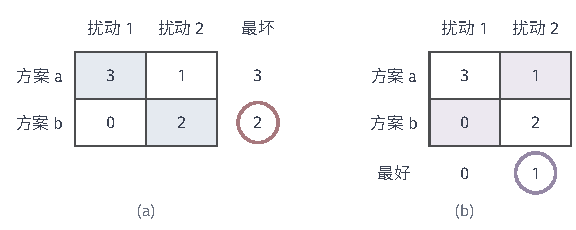
\includegraphics[width=97.5mm]{figures/05-optimization/07-multiple-criteria-and-nested-optimization/tikz/minimax-cost-table/figure.pdf}
 \caption{同一张代价表，两种决策顺序。(a)先定方案：每行取最大（蓝底），最坏列在表右，再在两个最坏值中取小，得到红圈中的$2$。(b)先定扰动：每列取最小（紫底），最好列在表下，再在两个最好值中取大，得到紫圈中的$1$。}
 \label{fig:minimax-cost-table}
\end{BookInlineFigure}

先定方案、再来扰动时，方案$\mathrm{a}$的最坏代价是$3$，方案$\mathrm{b}$的最坏代价是$2$，所以选$\mathrm{b}$，代价是$2$。这就是式~\eqref{eq:minimax-problem}的次序。

反过来，先定扰动、再选方案时，扰动$1$下最好的方案代价是$0$，扰动$2$下最好的方案代价是$1$。扰动一方要让代价大，所以选扰动$2$，代价是$1$。两个次序写成
\[
 \min_{\text{方案}}\max_{\text{扰动}}=2,\qquad\max_{\text{扰动}}\min_{\text{方案}}=1.
\]

同一张表给出两个不同的数。差别来自信息：后选的一方看得到先选的一方，可以对症下药。选方案的一方后选时代价是$1$，先选时代价是$2$，多出来的$1$是先亮底牌的代价。

后选不吃亏这件事不依赖具体的表。

\begin{lemma}[弱极小极大不等式]
\label{lem:minimax-weak}
对任意非空集合$\bm{X},\bm{Y}$和任意$f:\bm{X}\times\bm{Y}\to\mathbb{R}$，
\begin{equation}
 \sup_{\bm{y}\in\bm{Y}}\inf_{\bm{x}\in\bm{X}}f(\bm{x},\bm{y})\leq\inf_{\bm{x}\in\bm{X}}\sup_{\bm{y}\in\bm{Y}}f(\bm{x},\bm{y}).
 \label{eq:minimax-weak}
\end{equation}
\end{lemma}

\begin{proof}
任取$\bm{x}'\in\bm{X}$和$\bm{y}'\in\bm{Y}$。下确界不超过其中任何一项，上确界不小于其中任何一项，所以
\[
 \inf_{\bm{x}\in\bm{X}}f(\bm{x},\bm{y}')\leq f(\bm{x}',\bm{y}')\leq\sup_{\bm{y}\in\bm{Y}}f(\bm{x}',\bm{y}).
\]
最左端不含$\bm{x}'$，最右端不含$\bm{y}'$。左端对$\bm{y}'$取上确界，右端对$\bm{x}'$取下确界，不等号保持。
\end{proof}

连续的例子也一样。回到开头的$f(x,y)=(x-y)^2$，$X=\mathbb{R}$，$Y=[-1,1]$。固定$x$时，$f$是$y$的凸函数，最大值在端点取到，所以
\[
 \sup_{y\in[-1,1]}(x-y)^2=\max\{(x+1)^2,(x-1)^2\}=(\lvert x\rvert+1)^2.
\]

上式在$x=0$处最小，于是先定方案的值是$1$。反过来，无论$y$是多少，后选的$x$都可以取$x=y$，使代价为零，所以先定扰动的值是$0$。图~\ref{fig:minimax-worst-envelope}(a)里，外层最小化的是粗蓝线，而不是任何一条细线。

\begin{BookInlineFigure}
 \centering
 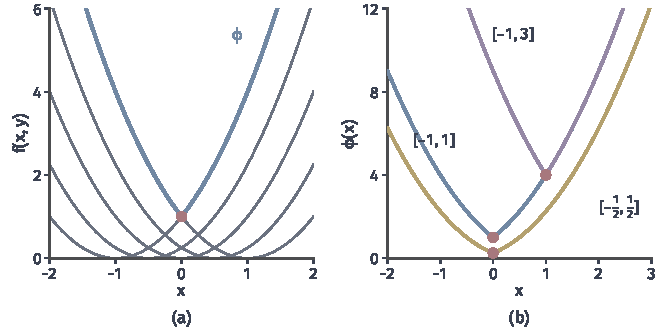
\includegraphics[width=112mm]{figures/05-optimization/07-multiple-criteria-and-nested-optimization/matplotlib/minimax-worst-envelope/figure.pdf}
 \caption{$f(x,y)=(x-y)^2$的最坏代价。(a)灰线是$y=0,\pm\frac12,\pm1$时的$f(\cdot,y)$，蓝线是它们对全部$y\in[-1,1]$的上边缘$\phi(x)=(\lvert x\rvert+1)^2$，红点是外层最优解。(b)三种响应集合下的最坏代价，黄线、蓝线、紫线分别对应标注的集合，红点是各自的最优解。集合$[-1,3]$把最优解移到了$x=1$。}
 \label{fig:minimax-worst-envelope}
\end{BookInlineFigure}

式~\eqref{eq:minimax-weak}的等号一般不成立，上面两个例子都严格小于。所以式~\eqref{eq:minimax-problem}里$\inf$和$\sup$的次序是问题的一部分，不能随手交换。交换需要额外的条件，第~\ref{sec:minimax-saddle}节专门研究。

\subsection{模型边界}
\label{sec:minimax-boundary}

极小极大的结论只对写进模型的$\bm{Y}$负责。“最坏”指的是集合$\bm{Y}$里最坏，集合之外的情形不在保证之内。

图~\ref{fig:minimax-worst-envelope}(b)比较了三个响应集合。对对称的集合$[-\rho,\rho]$，同样的计算给出最坏代价$(\lvert x\rvert+\rho)^2$，最优解都是$x=0$，最优值是$\rho^2$。集合放大时值变大，解却碰巧没动，这很容易让人以为解不依赖集合。

换成不对称的$Y=[-1,3]$，最坏代价变成
\[
 \max\{(x+1)^2,(x-3)^2\}.
\]
两条抛物线在$x=1$相交，最优解是$x=1$，最优值是$4$。按$Y=[-1,1]$选出的$x=0$，放到这个更大的集合下，最坏代价是$(0-3)^2=9$，比$4$差很多。一般地，$\bm{Y}_1\subseteq\bm{Y}_2$时内层上确界只会变大，所以小集合上的最坏值只是大集合上最坏值的下界，小集合上的最优解在大集合上没有任何保证。

\paragraph{Lagrange鞍点是特例}
第~\ref{chap:duality}章已经见过这种结构。约束问题的Lagrange函数$\mathcal{L}$对乘子取上确界时，可行点得到$f(\bm{x})$，不可行点得到$+\infty$，原问题因此写成
\[
 \inf_{\bm{x}\in\bm{D}}\ \sup_{\bm{\lambda}\geq\bm{0},\,\bm{\nu}}\ \mathcal{L}(\bm{x},\bm{\lambda},\bm{\nu}).
\]

这相当于在式~\eqref{eq:minimax-problem}中取$\bm{y}=(\bm{\lambda},\bm{\nu})$，$\bm{Y}=\mathbb{R}^m_{+}\times\mathbb{R}^p$，$\bm{X}=\bm{D}$。对偶问题是交换次序后的$\sup\inf$，弱对偶就是式~\eqref{eq:minimax-weak}。这个特例的结构比一般情形简单，$\mathcal{L}$关于$\bm{y}$是线性的，并且$\bm{Y}$由符号约束给出。本章的$f$不必有这种结构，$\bm{Y}$也可以是任意给定的集合。

\paragraph{本章不讨论的内容}
本章只有一个固定的代价$f$，$\bm{y}$只是“允许的响应”这个数学对象，不代表一个有自身偏好的决策者。模型中各方的偏好、均衡的解释和随时间展开的策略属于另一类问题，可参考\BookChapterRef{chap:static-games-equilibrium}{卷十第8章“静态博弈与均衡”}。这里只研究静态问题~\eqref{eq:minimax-problem}及其数值求解。

\section{最坏值函数}
\label{sec:minimax-value-function}

外层真正面对的目标是什么？本节把内层收进一个只依赖$\bm{x}$的函数，然后研究这个函数的性质，因为外层能用什么算法，全由这些性质决定。

\begin{definition}[最坏值函数]
\label{def:minimax-value}
称
\begin{equation}
 \phi(\bm{x})=\sup_{\bm{y}\in\bm{Y}}f(\bm{x},\bm{y})
 \label{eq:minimax-value}
\end{equation}
为\term{最坏值函数}（worst-case value function），它在某些点上可以取$+\infty$。上确界能够达到时，记最优响应的集合为
\begin{equation}
 \bm{Y}^\star(\bm{x})=\{\bm{y}\in\bm{Y}:f(\bm{x},\bm{y})=\phi(\bm{x})\}.
 \label{eq:minimax-response-set}
\end{equation}
\end{definition}

问题~\eqref{eq:minimax-problem}于是成为普通的单层问题$\inf_{\bm{x}\in\bm{X}}\phi(\bm{x})$。难点全部转移到了$\phi$上：它的每个函数值都要解一次最大化，它未必处处有限，也未必光滑。

有一点性质不需要任何计算。若对每个$\bm{y}\in\bm{Y}$，$f(\cdot,\bm{y})$都是凸函数，则$\phi$是凸函数，因为对任意$\theta\in[0,1]$，
\[
 f(\theta\bm{x}_1+(1-\theta)\bm{x}_2,\bm{y})\leq\theta f(\bm{x}_1,\bm{y})+(1-\theta)f(\bm{x}_2,\bm{y})\leq\theta\phi(\bm{x}_1)+(1-\theta)\phi(\bm{x}_2),
\]
再对$\bm{y}$取上确界即可。这里对$\bm{y}$一侧没有任何要求，$(x-y)^2$关于$y$是凸的，$\phi$照样是凸的。

内层可能出现三种不同的状况，它们影响的事情也不同，见表~\ref{tab:minimax-three-levels}。

\begin{BookInlineTable}
 \centering
 \begin{tabular}{@{}lll@{}}
  \toprule
  内层的状况 & 影响什么 & 反例\\
  \midrule
  最坏值有限 & 问题在该$\bm{x}$处是否有意义 & $f=xy$，$Y=\mathbb{R}$\\
  上确界达到 & 内层能否解出一个响应 & $f=x^2-e^{-y}$，$Y=\mathbb{R}$\\
  最优响应唯一 & 外层是否可微 & $f=xy$，$Y=[-1,1]$，$x=0$\\
  \bottomrule
 \end{tabular}
 \caption{内层的三种状况及其影响。反例说明相应性质可能失败。}
 \label{tab:minimax-three-levels}
\end{BookInlineTable}

第一行里，$x\neq0$时$\sup_{y\in\mathbb{R}}xy=+\infty$，只有$x=0$处最坏值有限。第二行里$\phi(x)=x^2$有限，但$-e^{-y}$在$y\to+\infty$时只是趋于$0$，没有哪个$y$达到上确界，内层的算法会一直往无穷远走。第三行里$x=0$时$f\equiv0$，每个$y$都是最优响应。

\subsection{响应切换}
\label{sec:minimax-switch}

光滑的$f$是否给出光滑的$\phi$？最简单的例子已经说明不会。取$f(x,y)=xy$，$Y=[-1,1]$。$f$关于$y$线性，最大值在端点，于是
\begin{equation}
 \phi(x)=\max\{x,-x\}=\lvert x\rvert.
 \label{eq:minimax-abs}
\end{equation}

每条直线$f(\cdot,y)$都光滑，它们的上边缘在原点却有折角，见图~\ref{fig:minimax-response-switch}(a)。原因是起作用的响应在$x=0$处换了人：$x>0$时最优响应是$y=1$，$x<0$时是$y=-1$。外层目标的尖点，正是内层最优响应切换的地方。这个切换与第~\ref{chap:nonsmooth-composite-optimization}章有限个函数取最大值时活跃分支的交替是同一个机制，只是这里的分支可能有无穷多条。

\begin{BookInlineFigure}
 \centering
 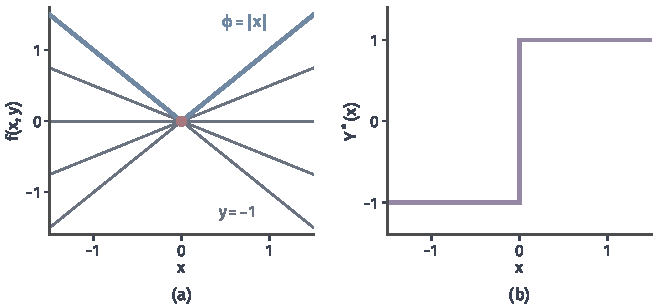
\includegraphics[width=112mm]{figures/05-optimization/07-multiple-criteria-and-nested-optimization/matplotlib/minimax-response-switch/figure.pdf}
 \caption{$f(x,y)=xy$，$Y=[-1,1]$。(a)灰线是$y=0,\pm\frac12,\pm1$时的直线，蓝线是上边缘$\phi(x)=\lvert x\rvert$，红点是外层最优解。(b)紫线是最优响应集合$Y^\star(x)$的图像，在$x=0$处是一整条竖直线段。}
 \label{fig:minimax-response-switch}
\end{BookInlineFigure}

图~\ref{fig:minimax-response-switch}(b)画出了$Y^\star(x)$。在$x\neq0$处它是单点，在$x=0$处是整个区间，这说明最优响应应当看作集合值映射。$(x-y)^2$的情形更极端：$Y^\star(0)=\{-1,1\}$是两个分开的点，集合甚至不连通。

下面的定理给出响应集合紧时能够保证的全部好性质。它说明响应集合可以跳，但图像是闭的，$\phi$本身仍然连续。

\begin{theorem}[紧响应集上的最坏值函数]
\label{thm:minimax-compact}
设$\bm{Y}$非空且紧，$f$在$\bm{X}\times\bm{Y}$上连续。则
\begin{enumerate}
 \item 对每个$\bm{x}\in\bm{X}$，上确界达到，$\bm{Y}^\star(\bm{x})$非空且紧；
 \item $\phi$在$\bm{X}$上有限且连续；
 \item 若$\bm{x}_k\to\bm{x}$，$\bm{y}_k\in\bm{Y}^\star(\bm{x}_k)$，$\bm{y}_k\to\bar{\bm{y}}$，则$\bar{\bm{y}}\in\bm{Y}^\star(\bm{x})$。
\end{enumerate}
\end{theorem}

\begin{proof}
第一条。$f(\bm{x},\cdot)$是紧集上的连续函数，最大值存在。$\bm{Y}^\star(\bm{x})$是连续函数$f(\bm{x},\cdot)$的水平集，是紧集$\bm{Y}$的闭子集，所以紧。

第二条。设$\bm{x}_k\to\bm{x}$。集合$\bm{K}=\{\bm{x}_k\}\cup\{\bm{x}\}$是紧的，$f$在紧集$\bm{K}\times\bm{Y}$上一致连续。记
\[
 \delta_k=\max_{\bm{y}\in\bm{Y}}\lvert f(\bm{x}_k,\bm{y})-f(\bm{x},\bm{y})\rvert\to0.
\]
对任意$\bm{y}$，有
\[
 f(\bm{x}_k,\bm{y})\leq f(\bm{x},\bm{y})+\delta_k\leq\phi(\bm{x})+\delta_k.
\]
对$\bm{y}$取最大，得到$\phi(\bm{x}_k)\leq\phi(\bm{x})+\delta_k$。交换$\bm{x}_k$与$\bm{x}$的角色，得到$\phi(\bm{x})\leq\phi(\bm{x}_k)+\delta_k$。所以$\phi(\bm{x}_k)\to\phi(\bm{x})$。

第三条。由$\bm{y}_k$的最优性，$f(\bm{x}_k,\bm{y}_k)=\phi(\bm{x}_k)$。令$k\to\infty$，用$f$和$\phi$的连续性，得到$f(\bm{x},\bar{\bm{y}})=\phi(\bm{x})$。
\end{proof}

第三条对应图~\ref{fig:minimax-response-switch}(b)的形状：从左右两侧趋于$x=0$时响应趋于$\pm1$，这两个极限都落在$Y^\star(0)$里。反过来不成立，$Y^\star(0)$中的$y=\frac12$不是任何邻近点响应的极限，所以这个映射不是连续的。

\subsection{值函数导数}
\label{sec:minimax-danskin}

要用梯度类方法更新$\bm{x}$，需要$\phi$的导数，而$\phi$本身没有显式表达式。能不能不微分内层的解？

看图~\ref{fig:minimax-danskin}(a)。在$x=0.5$处，起作用的是$y=-1$这条抛物线，上边缘在这里与它相切。切线的斜率就是这条抛物线在$x=0.5$处关于$x$的导数。$y$本身随$x$怎样变，在一阶上不起作用，因为$y$已经处在最优位置，朝任何可行方向挪动，代价都不会一阶增加。

第~\ref{chap:parametric-sensitivity}章的Danskin型结果给出了精确的说法。那里研究固定集合$\bm{C}$上的最优值函数$V(\bm{\theta})$，把它用到$-f$上，记号换成本章的，就得到下面的结论，证明见该章。

\begin{theorem}[最坏值函数的方向导数]
\label{thm:minimax-danskin}
设$\bm{X}\subseteq\mathbb{R}^{n}$开，$\bm{Y}$非空且紧，$f$与$\nabla_{\bm{x}}f$在$\bm{X}\times\bm{Y}$上连续。则对每个$\bm{x}\in\bm{X}$和方向$\bm{d}$，
\begin{equation}
 \phi'(\bm{x};\bm{d})=\max_{\bm{y}\in\bm{Y}^\star(\bm{x})}\bigl\langle\nabla_{\bm{x}}f(\bm{x},\bm{y}),\bm{d}\bigr\rangle.
 \label{eq:minimax-danskin}
\end{equation}
若$\bm{Y}^\star(\bm{x})=\{\bm{y}^\star(\bm{x})\}$是单点，则$\phi$在$\bm{x}$处可微，且
\begin{equation}
 \nabla\phi(\bm{x})=\nabla_{\bm{x}}f(\bm{x},\bm{y}^\star(\bm{x})).
 \label{eq:minimax-danskin-gradient}
\end{equation}
\end{theorem}

式~\eqref{eq:minimax-danskin}取最大值，是因为沿方向$\bm{d}$走一小步之后，起作用的是在这个方向上增长最快的那条响应。在开头的例子里，$\nabla_xf=2(x-y)$。$x=0.5$时响应唯一，$y^\star=-1$，式~\eqref{eq:minimax-danskin-gradient}给出
\[
 \phi'(0.5)=2(0.5+1)=3.
\]
它与直接求导$\phi'(x)=2(x+1)$的结果一致。

在$x=0$处，$Y^\star(0)=\{-1,1\}$，两个响应的偏导数是$2$和$-2$。式~\eqref{eq:minimax-danskin}给出
\[
 \phi'(0;d)=\max\{2d,-2d\}=2\lvert d\rvert.
\]
直接展开，得到
\[
 \phi(d)-\phi(0)=(\lvert d\rvert+1)^2-1=2\lvert d\rvert+d^2,
\]
一阶部分相同。

\begin{BookInlineFigure}
 \centering
 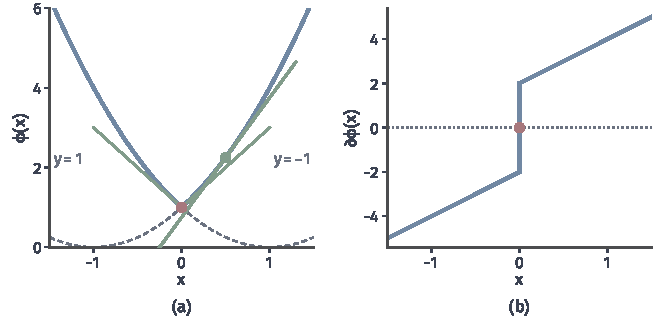
\includegraphics[width=112mm]{figures/05-optimization/07-multiple-criteria-and-nested-optimization/matplotlib/minimax-danskin/figure.pdf}
 \caption{$\phi(x)=(\lvert x\rvert+1)^2$的导数信息。(a)灰色虚线是$y=\pm1$两条抛物线，蓝线是上边缘。绿点$x=0.5$处只有一条活动响应，绿线是斜率为$3$的切线。红点$x=0$处两条响应同时活动，两段绿线的斜率是$\pm2$。(b)次微分的集值图像，在$x=0$处是竖直线段$[-2,2]$，它穿过点线$0$，说明$x=0$是最优解。}
 \label{fig:minimax-danskin}
\end{BookInlineFigure}

\paragraph{条件的作用}
定理要求响应集固定。这个条件去掉，公式就错了。取$f(x,y)=y$，让响应集随方案移动，$Y(x)=[-1,x]$，$x>-1$。则$\phi(x)=x$，导数是$1$，而$\partial f/\partial x\equiv0$。漏掉的部分来自集合边界的移动，要由乘子计入，这正是第~\ref{chap:parametric-sensitivity}章一般含参约束的内容。本章$\bm{Y}$不依赖$\bm{x}$，这个问题不出现。

紧性也不能省。$\bm{Y}$不紧时响应可能不存在，式~\eqref{eq:minimax-danskin}的右端失去意义，表~\ref{tab:minimax-three-levels}第二行就是这样。

\paragraph{关于$\bm{x}$凸时的次梯度集合}
多响应时只有方向导数还不够方便。若$f$关于$\bm{x}$凸，$\phi$是凸函数，可以用第~\ref{chap:nonsmooth-composite-optimization}章的次微分：$\bm{g}$是$\phi$在$\bm{x}$处的次梯度，指对所有$\bm{x}'$都有
\[
 \phi(\bm{x}')\geq\phi(\bm{x})+\langle\bm{g},\bm{x}'-\bm{x}\rangle.
\]

该章对有限个函数的最大值证明了次微分是活跃梯度的凸包，下面的定理把分支数推广到紧集上的无穷多个。

\begin{theorem}[最坏值函数的次微分]
\label{thm:minimax-subdiff}
设$\bm{X}=\mathbb{R}^{n}$，$\bm{Y}$非空且紧，$f$与$\nabla_{\bm{x}}f$连续，且对每个$\bm{y}\in\bm{Y}$，$f(\cdot,\bm{y})$是凸函数。则
\begin{equation}
 \partial\phi(\bm{x})=\operatorname{conv}\bigl\{\nabla_{\bm{x}}f(\bm{x},\bm{y}):\bm{y}\in\bm{Y}^\star(\bm{x})\bigr\}.
 \label{eq:minimax-subdiff}
\end{equation}
\end{theorem}

\begin{proof}
记右端为$\bm{K}$。$\bm{Y}^\star(\bm{x})$是紧集，它在连续映射$\nabla_{\bm{x}}f(\bm{x},\cdot)$下的像也是紧集，$\mathbb{R}^n$中紧集的凸包仍是紧集，所以$\bm{K}$紧且凸。

先证$\bm{K}\subseteq\partial\phi(\bm{x})$。任取$\bm{y}\in\bm{Y}^\star(\bm{x})$和$\bm{x}'$。由$\phi$的定义和$f(\cdot,\bm{y})$的凸性，
\[
 \phi(\bm{x}')\geq f(\bm{x}',\bm{y})\geq f(\bm{x},\bm{y})+\langle\nabla_{\bm{x}}f(\bm{x},\bm{y}),\bm{x}'-\bm{x}\rangle.
\]
左边第二项的$f(\bm{x},\bm{y})$等于$\phi(\bm{x})$。把这样的不等式按凸组合的权重相加，右端的向量就换成了$\bm{K}$中的任意元素。

再证反向。设$\bm{g}\in\partial\phi(\bm{x})$但$\bm{g}\notin\bm{K}$。$\bm{K}$非空、闭、凸，由第~\ref{chap:duality}章点与闭凸集的严格分离，存在$\bm{d}$，使
\[
 \langle\bm{g},\bm{d}\rangle>\max_{\bm{c}\in\bm{K}}\langle\bm{c},\bm{d}\rangle\geq\max_{\bm{y}\in\bm{Y}^\star(\bm{x})}\langle\nabla_{\bm{x}}f(\bm{x},\bm{y}),\bm{d}\rangle=\phi'(\bm{x};\bm{d}).
\]
最后的等号是式~\eqref{eq:minimax-danskin}。

另一方面，次梯度不等式给出
\[
 \phi(\bm{x}+s\bm{d})-\phi(\bm{x})\geq s\langle\bm{g},\bm{d}\rangle.
\]
除以$s>0$并令$s\downarrow0$，得到
\[
 \phi'(\bm{x};\bm{d})\geq\langle\bm{g},\bm{d}\rangle.
\]
这与上式矛盾。
\end{proof}

对开头的例子，活动偏导数是$\pm2$，所以$\partial\phi(0)=[-2,2]$，见图~\ref{fig:minimax-danskin}(b)。对$f=xy$，活动偏导数是$\lvert y\rvert\leq1$的全体$y$，所以$\partial\phi(0)=[-1,1]$。两者都含$0$，所以$x=0$都是全局最优解。

多响应时要注意一件事：只取其中一个响应，它给出的梯度未必是下降方向。在$(x-y)^2$的$x=0$处，取$y=1$，偏导数是$-2$，沿负偏导数方向是把$x$往正的方向移，而$\phi$沿这个方向是上升的。这和第~\ref{chap:nonsmooth-composite-optimization}章次梯度的负方向未必下降是同一回事。值函数的导数和次梯度只回答“外层目标对$\bm{x}$怎样变化”；$\bm{Y}$或约束也随参数变化时的完整敏感性，由第~\ref{chap:parametric-sensitivity}章处理。

\section{鞍点}
\label{sec:minimax-saddle}

判断一个$\bm{x}$好不好，要算$\phi(\bm{x})$，也就要解一次内层。如果手上同时有一个$\bm{x}$和一个$\bm{y}$，能不能让它们互相作证？本节研究这样一对候选应当满足什么关系，它和两个次序的值有什么联系。

记交换次序后的函数为
\begin{equation}
 \psi(\bm{y})=\inf_{\bm{x}\in\bm{X}}f(\bm{x},\bm{y}),
 \label{eq:minimax-psi}
\end{equation}
它是$\bm{y}$先定时外层能做到的最好代价。两个次序的值分别记作
\begin{equation}
 \bar{v}=\inf_{\bm{x}\in\bm{X}}\phi(\bm{x}),\qquad\underline{v}=\sup_{\bm{y}\in\bm{Y}}\psi(\bm{y}).
 \label{eq:minimax-values}
\end{equation}
式~\eqref{eq:minimax-weak}就是$\underline{v}\leq\bar{v}$。

想象一个山口。沿着山脊方向，山口是最低点；沿着翻山的方向，山口是最高点。站在山口，往山脊两头走都要上坡，往两侧山谷走都要下坡。下面的定义把这个图景用到两组变量上：沿$\bm{x}$的方向山口最低，沿$\bm{y}$的方向山口最高。

\begin{definition}[全局鞍点]
\label{def:minimax-saddle}
若$(\bm{x}^\star,\bm{y}^\star)\in\bm{X}\times\bm{Y}$对所有$\bm{x}\in\bm{X}$，$\bm{y}\in\bm{Y}$满足
\begin{equation}
 f(\bm{x}^\star,\bm{y})\leq f(\bm{x}^\star,\bm{y}^\star)\leq f(\bm{x},\bm{y}^\star),
 \label{eq:minimax-saddle}
\end{equation}
就称它是$f$在$\bm{X}\times\bm{Y}$上的\term{全局鞍点}（global saddle point）。
\end{definition}

式~\eqref{eq:minimax-saddle}的右半边说，固定$\bm{y}^\star$时$\bm{x}^\star$全局最小；左半边说，固定$\bm{x}^\star$时$\bm{y}^\star$全局最大。任何一侧单独改变，都不能改善自己的目标。山口的类比在这里到头了：山的形状只有一种，而鞍点还取决于哪个变量要最小化、哪个要最大化。

这个定义比第~\ref{chap:saddle-points}章的鞍点多了分工。那一章的鞍点指Hessian不定的驻点，只看函数形状，不问变量的角色。

要把几个相近的概念分开，看图~\ref{fig:minimax-saddle-types}中的三个二次函数，以及后面一个四次函数。$x$是外层变量，$y$是内层变量。

\begin{BookInlineFigure}
 \centering
 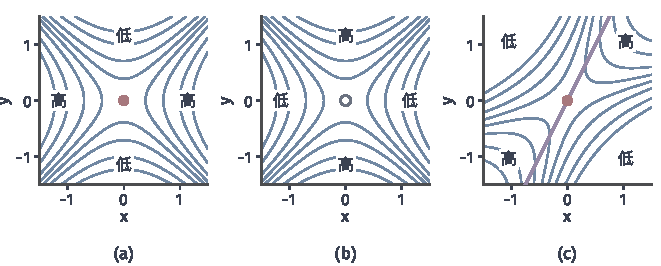
\includegraphics[width=112mm]{figures/05-optimization/07-multiple-criteria-and-nested-optimization/matplotlib/minimax-saddle-types/figure.pdf}
 \caption{原点都是两侧一阶驻定点，蓝线是等高线，“高”“低”标出函数值的高低区域。(a)$x^2-y^2$：沿$x$最小、沿$y$最大，红点是全局鞍点。(b)$y^2-x^2$：形状相同而角色相反，空心点既不是鞍点，也不解决顺序问题。(c)$-\frac12x^2+2xy-\frac12y^2$：紫线是最优响应$y=2x$，红点解决顺序问题，却不是鞍点。}
 \label{fig:minimax-saddle-types}
\end{BookInlineFigure}

(a)的$f=x^2-y^2$在全平面满足式~\eqref{eq:minimax-saddle}，原点是全局鞍点。(b)的$f=y^2-x^2$在原点的两个偏导数也都为零，但固定$y=0$时$-x^2$在$x=0$处最大，外层变量离开原点反而更好。

(c)最值得留意。取$f=-\frac12x^2+2xy-\frac12y^2$，$X=Y=\mathbb{R}$。这个函数在本章后面反复使用。内层关于$y$严格凹，令$\partial_yf=2x-y=0$，得$y^\star(x)=2x$。代回得到
\begin{equation}
 \phi(x)=-\frac12x^2+4x^2-2x^2=\frac32x^2.
 \label{eq:minimax-running-phi}
\end{equation}

$\phi$的最小点是$x=0$，顺序问题的解是原点，值是$0$。可是固定$y=0$时$f(x,0)=-\frac12x^2$在$x=0$处最大，式~\eqref{eq:minimax-saddle}的右半边不成立。对任意$y$，$\psi(y)=\inf_xf=-\infty$，所以$\underline{v}=-\infty<0=\bar{v}$。外层在这里不是对$\bm{x}$最小化固定的$f$，它考虑的是$y$会跟着$x$一起变，这个跟随效应把$-\frac12x^2$的向下弯曲翻了过来。

局部的版本是把式~\eqref{eq:minimax-saddle}中的“所有”改成“$(\bm{x}^\star,\bm{y}^\star)$某个邻域内的所有”，称为\term{局部鞍点}（local saddle point）。例如在$X=[-3,3]$，$Y=[-1,1]$上取
\begin{equation}
 f(x,y)=x^2-\frac14x^4-y^2.
 \label{eq:minimax-local-saddle}
\end{equation}
在原点附近$x^2-\frac14x^4\geq0$，所以原点是局部鞍点。但$f(3,0)=9-\frac{81}{4}=-11.25<0$，外层变量跑远了反而更好，所以原点不是全局鞍点。

\begin{BookInlineTable}
 \centering
 \begin{tabular}{@{}lll@{}}
  \toprule
  概念 & 要求 & 例子\\
  \midrule
  两侧一阶驻定 & 无约束时两个偏梯度为零 & 图~\ref{fig:minimax-saddle-types}三个原点\\
  局部鞍点 & 式~\eqref{eq:minimax-saddle}在邻域内成立 & 式~\eqref{eq:minimax-local-saddle}的原点\\
  全局鞍点 & 式~\eqref{eq:minimax-saddle}在全域成立 & $x^2-y^2$的原点\\
  顺序问题的解 & $\bm{x}$最小化$\phi$ & 图~\ref{fig:minimax-saddle-types}(c)的原点\\
  \bottomrule
 \end{tabular}
 \caption{四个相近概念的比较。两侧一阶驻定最弱，它不自动解决顺序问题；顺序问题的解也不一定是鞍点。}
 \label{tab:minimax-saddle-compare}
\end{BookInlineTable}

全局鞍点与两个次序的关系，由下面的定理给出。

\begin{theorem}[鞍点与最值相等]
\label{thm:minimax-saddle-values}
设$\bm{x}^\star\in\bm{X}$，$\bm{y}^\star\in\bm{Y}$。$(\bm{x}^\star,\bm{y}^\star)$是全局鞍点，当且仅当同时满足
\begin{equation}
 \phi(\bm{x}^\star)=\bar{v},\qquad\psi(\bm{y}^\star)=\underline{v},\qquad\bar{v}=\underline{v}\in\mathbb{R}.
 \label{eq:minimax-saddle-values}
\end{equation}
此时共同的值等于$f(\bm{x}^\star,\bm{y}^\star)$。
\end{theorem}

\begin{proof}
必要性。对式~\eqref{eq:minimax-saddle}的左半边取$\bm{y}$的上确界，右半边取$\bm{x}$的下确界，得到
\[
 \phi(\bm{x}^\star)\leq f(\bm{x}^\star,\bm{y}^\star)\leq\psi(\bm{y}^\star).
\]
结合定义，又有
\[
 \underline{v}\leq\bar{v}\leq\phi(\bm{x}^\star),\qquad\psi(\bm{y}^\star)\leq\underline{v}.
\]
把这些不等式连起来，就成为一个闭环，其中所有的量都相等。

充分性。由式~\eqref{eq:minimax-saddle-values}，$\phi(\bm{x}^\star)=\psi(\bm{y}^\star)$是有限数。定义给出
\[
 \psi(\bm{y}^\star)\leq f(\bm{x}^\star,\bm{y}^\star)\leq\phi(\bm{x}^\star),
\]
所以三者相等。于是对任意$\bm{x},\bm{y}$，
\[
 f(\bm{x}^\star,\bm{y})\leq\phi(\bm{x}^\star)=\psi(\bm{y}^\star)\leq f(\bm{x},\bm{y}^\star),
\]
中间的值等于$f(\bm{x}^\star,\bm{y}^\star)$，这就是式~\eqref{eq:minimax-saddle}。
\end{proof}

定理说明鞍点集合是一个乘积集合。若$(\bm{x}_1,\bm{y}_1)$和$(\bm{x}_2,\bm{y}_2)$都是鞍点，式~\eqref{eq:minimax-saddle-values}的三条对$(\bm{x}_1,\bm{y}_2)$同样成立，所以它也是鞍点，不需要把两侧配对寻找。这与第~\ref{chap:duality}章的Lagrange鞍点定理一致，那里的$\mathcal{L}$就是这里的$f$。

\subsection{最值交换}
\label{sec:minimax-exchange}

什么条件能让$\underline{v}=\bar{v}$？先回到图~\ref{fig:minimax-cost-table}的代价表，看一个修复办法。两个次序之所以不同，是因为每一方只能选一个端点。设想方案可以按比例组合：把份额$p$投给方案$\mathrm{a}$，$1-p$投给方案$\mathrm{b}$；扰动也按比例$q$和$1-q$作用，代价按份额加权。

记$p,q\in[0,1]$，代价为
\[
 f(p,q)=3pq+p(1-q)+2(1-p)(1-q).
\]
展开并配方，得到
\begin{equation}
 f(p,q)=4pq-p-2q+2=4\Bigl(p-\frac12\Bigr)\Bigl(q-\frac14\Bigr)+\frac32.
 \label{eq:minimax-relaxed}
\end{equation}

$f$关于$q$是线性的，最大值在端点取到，所以
\[
 \phi(p)=\max\{f(p,0),f(p,1)\}=\max\{2-p,3p\}.
\]
同理，$f$关于$p$线性，最小值在端点取到，所以
\[
 \psi(q)=\min\{f(0,q),f(1,q)\}=\min\{2-2q,1+2q\}.
\]

$\phi$在$2-p=3p$即$p=\frac12$处最小，$\psi$在$2-2q=1+2q$即$q=\frac14$处最大，并且
\[
 \phi\Bigl(\frac12\Bigr)=\psi\Bigl(\frac14\Bigr)=\frac32.
\]
由定理~\ref{thm:minimax-saddle-values}，$(\frac12,\frac14)$是鞍点，见图~\ref{fig:minimax-relaxed-table}。两个次序现在给出同一个值$\frac32$，它落在原来的$1$和$2$之间。允许按比例组合，也就是把问题做成关于各自变量线性的，先后的差别消失了。

\begin{BookInlineFigure}
 \centering
 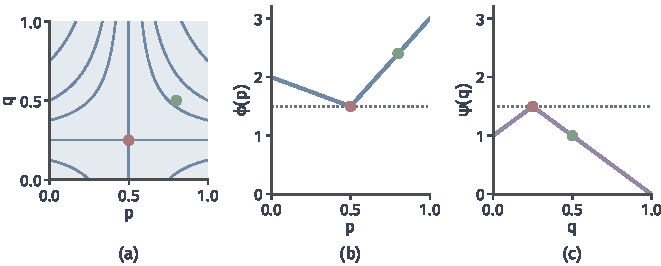
\includegraphics[width=112mm]{figures/05-optimization/07-multiple-criteria-and-nested-optimization/matplotlib/minimax-relaxed-table/figure.pdf}
 \caption{代价表的比例松弛$f(p,q)=4(p-\frac12)(q-\frac14)+\frac32$。(a)浅蓝是可行域，蓝线是等高线，穿过红点的十字是值为$\frac32$的等高线，红点是鞍点，绿点是候选$(0.8,0.5)$。(b)外层目标$\phi(p)$，红点是最小点。(c)$\psi(q)$，红点是最大点。点线是共同的值$\frac32$，绿点是候选在两条曲线上的值。}
 \label{fig:minimax-relaxed-table}
\end{BookInlineFigure}

这个例子的结构可以一般化：两个集合都是紧凸集，$f$关于$\bm{x}$凸、关于$\bm{y}$凹。凸凹性是说，混合之后不会比原来更有利于对面。

\begin{theorem}[紧集上的极小极大定理]
\label{thm:minimax-theorem}
设$\bm{X},\bm{Y}$非空、紧、凸，$f$在$\bm{X}\times\bm{Y}$上连续；对每个$\bm{y}\in\bm{Y}$，$f(\cdot,\bm{y})$是凸函数；对每个$\bm{x}\in\bm{X}$，$f(\bm{x},\cdot)$是凹函数。则
\begin{equation}
 \min_{\bm{x}\in\bm{X}}\max_{\bm{y}\in\bm{Y}}f(\bm{x},\bm{y})=\max_{\bm{y}\in\bm{Y}}\min_{\bm{x}\in\bm{X}}f(\bm{x},\bm{y}),
 \label{eq:minimax-theorem}
\end{equation}
两侧的最值都达到，并且存在全局鞍点。
\end{theorem}

\begin{proof}
由式~\eqref{eq:minimax-weak}，只需排除$\underline{v}<\bar{v}$。用反证法，设$\underline{v}<\bar{v}$，取实数$c$满足$\underline{v}<c<\bar{v}$。

第一步，把无穷多个$\bm{y}$化成有限个。对每个$\bm{x}\in\bm{X}$，有$\phi(\bm{x})\geq\bar{v}>c$，所以存在$\bm{y}$使$f(\bm{x},\bm{y})>c$。于是开集族
\[
 \bm{U}_{\bm{y}}=\{\bm{x}\in\bm{X}:f(\bm{x},\bm{y})>c\},\qquad\bm{y}\in\bm{Y}
\]
覆盖了$\bm{X}$。$\bm{X}$是紧集，存在有限个$\bm{y}_1,\ldots,\bm{y}_k$，使每个$\bm{x}\in\bm{X}$都至少满足一条$f(\bm{x},\bm{y}_i)>c$。

第二步，用凸性分离出权重。令
\[
 \bm{S}=\bigl\{\bm{w}\in\mathbb{R}^k:\text{存在}\ \bm{x}\in\bm{X},\ \text{使}\ w_i\geq f(\bm{x},\bm{y}_i)\ \text{对所有}\ i\ \text{成立}\bigr\}.
\]
$\bm{X}$是凸集，每个$f(\cdot,\bm{y}_i)$是凸函数，所以$\bm{S}$是凸集。点$\bm{c}=(c,\ldots,c)$不在$\bm{S}$中，否则某个$\bm{x}$使所有$f(\bm{x},\bm{y}_i)\leq c$，与第一步矛盾。

第~\ref{chap:duality}章的点与凸集分离引理不要求$\bm{S}$闭，由它得到$\bm{a}\neq\bm{0}$，使
\[
 \langle\bm{a},\bm{w}\rangle\geq\langle\bm{a},\bm{c}\rangle\qquad\text{对所有}\ \bm{w}\in\bm{S}.
\]
$\bm{S}$中的点把任一分量增大后仍在$\bm{S}$中。若某个$a_i<0$，让$w_i\to+\infty$，左端趋于$-\infty$，矛盾。所以$\bm{a}\geq\bm{0}$，可以归一化为$\sum_ia_i=1$，此时$\langle\bm{a},\bm{c}\rangle=c$。

对任意$\bm{x}\in\bm{X}$，取$w_i=f(\bm{x},\bm{y}_i)$，得到
\[
 \sum_{i=1}^ka_if(\bm{x},\bm{y}_i)\geq c.
\]

第三步，用凹性把有限个$\bm{y}_i$合成一个。令$\bar{\bm{y}}=\sum_ia_i\bm{y}_i$。$\bm{Y}$是凸集，所以$\bar{\bm{y}}\in\bm{Y}$。$f(\bm{x},\cdot)$是凹函数，所以对所有$\bm{x}\in\bm{X}$，
\[
 f(\bm{x},\bar{\bm{y}})\geq\sum_{i=1}^ka_if(\bm{x},\bm{y}_i)\geq c.
\]
于是$\psi(\bar{\bm{y}})\geq c>\underline{v}$，与$\underline{v}$是$\psi$的上确界矛盾。所以$\underline{v}=\bar{v}$。

最后看达到。由定理~\ref{thm:minimax-compact}，$\phi$在紧集$\bm{X}$上连续，最小值达到；对$-f$用同一定理，$\psi$在紧集$\bm{Y}$上连续，最大值达到。取最优点$\bm{x}^\star,\bm{y}^\star$，由定理~\ref{thm:minimax-saddle-values}，它们组成全局鞍点。
\end{proof}

证明里每个条件各有职责。$\bm{X}$紧把无穷多个响应化为有限个；关于$\bm{x}$的凸性使$\bm{S}$凸，因而能分离出权重；关于$\bm{y}$的凹性与$\bm{Y}$的凸性把“按权重混合的$\bm{y}_i$”合成$\bm{Y}$中的一个点。开头的$(x-y)^2$缺的是最后一条：$f$关于$y$是凸的，端点$y=\pm1$按等权混合的代价是$x^2+1$，而单点$y=0$的代价只有$x^2$，混合无法用一个$y$代替。

\paragraph{放宽紧性时要分别核对}
更一般的Sion定理只要求其中一个集合紧，把凸凹性放宽为拟凸拟凹，连续性放宽为半连续，结论仍是两个次序的值相等\scite{sion1958}。它的证明需要一套关于水平集连通性的论证，篇幅较长。这里用两个例子说明放宽之后什么会失去。

两个集合都不紧时，值可能不相等。在$X=Y=[0,\infty)$上取
\[
 f(x,y)=\frac{y-x}{1+x+y}.
\]
由于$f=-1+\frac{1+2y}{1+x+y}$，它关于$x$凸；由于$f=1-\frac{1+2x}{1+x+y}$，它关于$y$凹。令$y\to\infty$得$\phi(x)=1$，令$x\to\infty$得$\psi(y)=-1$，所以$\bar{v}=1$，$\underline{v}=-1$。这里凸凹性和连续性都有，只是少了紧性，见图~\ref{fig:minimax-exchange-fail}(a)。

值相等也不等于鞍点存在。在$X=[0,\infty)$，$Y=[0,1]$上取$f(x,y)=ye^{-x}$，满足Sion定理的条件。内层取$y=1$，得$\phi(x)=e^{-x}$，它的下确界是$0$，但没有$x$取到；外层令$x\to\infty$，得$\psi(y)=0$。所以$\bar{v}=\underline{v}=0$，而没有$x$使$\phi(x)=0$，由定理~\ref{thm:minimax-saddle-values}，鞍点不存在，见图~\ref{fig:minimax-exchange-fail}(b)。

\begin{BookInlineFigure}
 \centering
 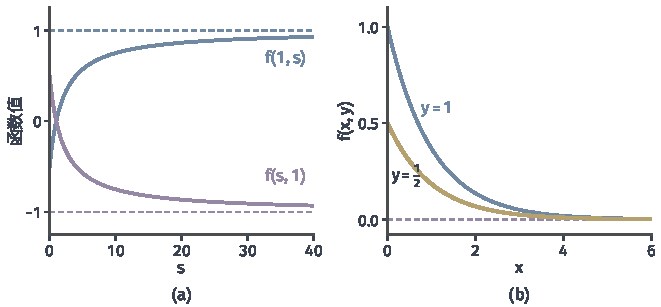
\includegraphics[width=112mm]{figures/05-optimization/07-multiple-criteria-and-nested-optimization/matplotlib/minimax-exchange-fail/figure.pdf}
 \caption{放宽紧性的两种后果。(a)$f=(y-x)/(1+x+y)$在$[0,\infty)^2$上：蓝线$f(1,s)$沿$y=s$趋于蓝色虚线$1$，紫线$f(s,1)$沿$x=s$趋于紫色虚线$-1$，两个次序的值不同。(b)$f=ye^{-x}$：蓝线和黄线分别是$y=1,\frac12$时的截线，都趋于紫色虚线$0$而取不到，值相等但没有鞍点。}
 \label{fig:minimax-exchange-fail}
\end{BookInlineFigure}

最值相等是一个关于数的结论。要从中取出一对点，还必须分别核对$\phi$的最小值和$\psi$的最大值是否达到。

\subsection{鞍点间隙}
\label{sec:minimax-gap}

有了$\phi$和$\psi$，就能给任何一对可行候选打分。这是第~\ref{chap:duality}章“可行点给上界、乘子给下界”的直接推广。

\begin{definition}[鞍点间隙]
\label{def:minimax-gap}
对$(\bm{x},\bm{y})\in\bm{X}\times\bm{Y}$，定义
\begin{equation}
 G(\bm{x},\bm{y})=\sup_{\bm{v}\in\bm{Y}}f(\bm{x},\bm{v})-\inf_{\bm{u}\in\bm{X}}f(\bm{u},\bm{y})=\phi(\bm{x})-\psi(\bm{y}),
 \label{eq:minimax-gap}
\end{equation}
称为\term{鞍点间隙}（saddle gap），其中$\phi(\bm{x})=+\infty$或$\psi(\bm{y})=-\infty$时$G=+\infty$。
\end{definition}

间隙度量的是：固定对方，各自还能改善多少，两边加起来。

\begin{theorem}[间隙是全局证书]
\label{thm:minimax-gap}
对任意$(\bm{x},\bm{y})\in\bm{X}\times\bm{Y}$，只要$G(\bm{x},\bm{y})$有定义，就有$G(\bm{x},\bm{y})\geq\bar{v}-\underline{v}\geq0$，并且
\begin{equation}
 \phi(\bm{x})-\bar{v}\leq G(\bm{x},\bm{y}),\qquad\underline{v}-\psi(\bm{y})\leq G(\bm{x},\bm{y}).
 \label{eq:minimax-gap-bound}
\end{equation}
当$G(\bm{x},\bm{y})$有限时，$G(\bm{x},\bm{y})=0$当且仅当$(\bm{x},\bm{y})$是全局鞍点。
\end{theorem}

\begin{proof}
由定义，$\phi(\bm{x})\geq\bar{v}$，$\psi(\bm{y})\leq\underline{v}$，相减得$G\geq\bar{v}-\underline{v}$，它由式~\eqref{eq:minimax-weak}非负。

式~\eqref{eq:minimax-gap-bound}的第一式等价于$\psi(\bm{y})\leq\bar{v}$，它由$\psi(\bm{y})\leq\underline{v}\leq\bar{v}$得到。第二式等价于$\underline{v}\leq\phi(\bm{x})$，它由$\underline{v}\leq\bar{v}\leq\phi(\bm{x})$得到。

若$G=0$，由上面的不等式，$\phi(\bm{x})=\bar{v}$，$\psi(\bm{y})=\underline{v}$，且$\bar{v}=\underline{v}$，由定理~\ref{thm:minimax-saddle-values}它是全局鞍点。反过来，全局鞍点满足式~\eqref{eq:minimax-saddle-values}，相减为零。
\end{proof}

式~\eqref{eq:minimax-gap-bound}是最有用的部分。它不需要知道$\bar{v}$，就能说出$\bm{x}$的最坏值离最优最多差多少。回到比例松弛，取图~\ref{fig:minimax-relaxed-table}的绿点$(p,q)=(0.8,0.5)$，算得
\[
 \phi(0.8)=\max\{1.2,2.4\}=2.4,\qquad\psi(0.5)=\min\{1,2\}=1.
\]
所以
\[
 G(0.8,0.5)=1.4.
\]
真实的次优量是$\phi(0.8)-\frac32=0.9$，确实不超过$1.4$。

对$f=xy$，$X=Y=[-1,1]$，有
\begin{equation}
 \phi(x)=\lvert x\rvert,\qquad\psi(y)=-\lvert y\rvert,\qquad G(x,y)=\lvert x\rvert+\lvert y\rvert.
 \label{eq:minimax-box-gap}
\end{equation}
这个例子的答案可以直接读出来，后面却会看到，最直接的算法在它上面就会失败。

\paragraph{非紧域上的间隙}
把上面的集合换成$X=Y=\mathbb{R}$，同一个$f=xy$的$\phi(x)$在$x\neq0$时是$+\infty$，于是$G$除了原点处处是$+\infty$。此时$G$虽然没有错，却完全不能区分候选的好坏。

常见的处理是只在一个有界区域$\bm{B}=\bm{B}_{\bm{X}}\times\bm{B}_{\bm{Y}}$上取极值，其中$\bm{B}_{\bm{X}}\subseteq\bm{X}$，$\bm{B}_{\bm{Y}}\subseteq\bm{Y}$，候选在$\bm{B}$内，得到
\begin{equation}
 G_{\bm{B}}(\bm{x},\bm{y})=\sup_{\bm{v}\in\bm{B}_{\bm{Y}}}f(\bm{x},\bm{v})-\inf_{\bm{u}\in\bm{B}_{\bm{X}}}f(\bm{u},\bm{y}).
 \label{eq:minimax-restricted-gap}
\end{equation}

称为\term{限定间隙}（restricted gap）。上确界和下确界的范围变小，所以$G_{\bm{B}}\leq G$。它是真实间隙的下估计，小的$G_{\bm{B}}$不能说明$G$小。

式~\eqref{eq:minimax-local-saddle}正好说明这一点。取$\bm{B}=[-1,1]\times[-1,1]$，候选为原点。在$\bm{B}$内$x^2-\frac14x^4\geq0$，$-y^2\leq0$，所以$G_{\bm{B}}(0,0)=0$。但在整个$X=[-3,3]$上，
\[
 \psi(0)=\min_{\lvert u\rvert\leq3}\Bigl(u^2-\frac14u^4\Bigr)=-11.25,\qquad\phi(0)=0.
\]
所以真实间隙是$11.25$，见图~\ref{fig:minimax-restricted-gap}。局部检验框看不到框外的低谷，零的限定间隙不能当作全局证书。

\begin{BookInlineFigure}
 \centering
 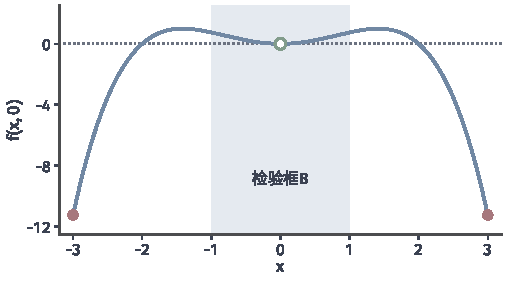
\includegraphics[width=86mm]{figures/05-optimization/07-multiple-criteria-and-nested-optimization/matplotlib/minimax-restricted-gap/figure.pdf}
 \caption{$f(x,y)=x^2-\frac14x^4-y^2$在$y=0$上的截线，$X=[-3,3]$。浅蓝区域是检验框，框内原点（绿色空心点）的值最小，限定间隙为零。红点是框外的真正最小点，值为$-11.25$，真实间隙是$11.25$。}
 \label{fig:minimax-restricted-gap}
\end{BookInlineFigure}

凸凹问题里限定间隙的意义强一些。若$\bm{B}$内含有一个全局鞍点$(\bm{x}^\star,\bm{y}^\star)$，则
\[
 G_{\bm{B}}(\bm{x},\bm{y})\geq f(\bm{x},\bm{y}^\star)-f(\bm{x}^\star,\bm{y})\geq0,
\]
所以它至少是一个非负的度量，只要$\bm{B}$足够大，把解包含在内。这条依赖“$\bm{B}$内含解”这个事实，而这个事实本身需要另外的证据。

\section{内层响应法}
\label{sec:minimax-inner-response}

最直接的求解办法是照着决策顺序来：固定当前的$\bm{x}$，先求最坏响应，再用值函数的信息更新$\bm{x}$。外层用什么算法，前面各章已经讲过，本节只回答两个新问题：内层要解到什么程度，内层的误差怎样传到外层。

图~\ref{fig:minimax-response-flow}是整个方法的结构。

\begin{BookInlineFigure}
 \centering
 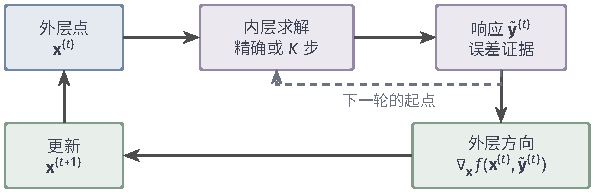
\includegraphics[width=100.7mm]{figures/05-optimization/07-multiple-criteria-and-nested-optimization/tikz/minimax-response-flow/figure.pdf}
 \caption{内层响应法的一轮。紫框是内层计算，绿框是外层计算。内层的输出除了响应，还应带有它的误差证据。虚线表示本轮响应作为下一轮内层的起点。}
 \label{fig:minimax-response-flow}
\end{BookInlineFigure}

\subsection{精确响应}
\label{sec:minimax-exact-response}

\paragraph{主要思想}
设内层最优响应唯一且$\phi$可微。定理~\ref{thm:minimax-danskin}说，算梯度时可以把响应当作常数，所以外层的梯度步就是
\begin{equation}
 \bm{x}^{(t+1)}=P_{\bm{X}}\Bigl(\bm{x}^{(t)}-\alpha\nabla_{\bm{x}}f\bigl(\bm{x}^{(t)},\bm{y}^\star(\bm{x}^{(t)})\bigr)\Bigr),
 \label{eq:minimax-exact-step}
\end{equation}
其中$\bm{X}$是闭凸集，$P_{\bm{X}}$是第~\ref{chap:feasible-iterations}章的欧氏投影，$\bm{X}=\mathbb{R}^n$时投影是恒等映射。这就是对$\phi$做投影梯度法，收敛性由$\phi$的光滑常数和凸性决定，不需要新的理论。

\paragraph{计算过程}
用式~\eqref{eq:minimax-running-phi}的函数演示，$f=-\frac12x^2+2xy-\frac12y^2$，$X=Y=\mathbb{R}$。

\needspace{6\baselineskip}
\paragraph{变量}
\begin{itemize}
 \item $x^{(t)}$：外层变量；
 \item $y^{(t)}$：内层在$x^{(t)}$处的精确响应；
 \item $g^{(t)}$：外层偏导数；
 \item $\alpha>0$：外层步长。
\end{itemize}

\paragraph{初始化}
取$x^{(0)}$。例中$x^{(0)}=1$，步长$\alpha=\frac16$，当$\lvert g^{(t)}\rvert\leq0.4$时停止。

\needspace{6\baselineskip}
\paragraph{每轮更新}
\begin{enumerate}
 \item 解内层，得$y^{(t)}=y^\star(x^{(t)})$。例中$y^\star(x)=2x$，第一轮
 \[
  y^{(0)}=2.
 \]
 \item 计算外层偏导数$g^{(t)}=\partial_xf(x^{(t)},y^{(t)})$。例中$\partial_xf=-x+2y$，第一轮
 \[
  g^{(0)}=-1+4=3.
 \]
 \item 由式~\eqref{eq:minimax-exact-step}更新。例中第一轮
 \[
  x^{(1)}=1-\frac16\cdot3=\frac12.
 \]
\end{enumerate}

第二轮$y^{(1)}=1$，$g^{(1)}=\frac32$，$x^{(2)}=\frac14$。第三轮$y^{(2)}=\frac12$，$g^{(2)}=\frac34$，$x^{(3)}=\frac18$。第四轮$y^{(3)}=\frac14$，$g^{(3)}=\frac38\leq0.4$，停止。

最终得到$x^{(3)}=\frac18$，最坏值$\phi(\frac18)=\frac{3}{128}$。例中$g^{(t)}=\phi'(x^{(t)})=3x^{(t)}$，与式~\eqref{eq:minimax-running-phi}的导数相同，这正是定理~\ref{thm:minimax-danskin}的内容。

\paragraph{响应切换时改用非光滑方法}
$\phi$有折角时，式~\eqref{eq:minimax-exact-step}里的偏梯度只是一个次梯度，而次梯度不随接近解而变小。设$f=(x-y)^2$，$Y=[-1,1]$，$x^{(0)}=0.8$，固定步长$\alpha=0.2$。

$x>0$时最坏响应是$y=-1$，偏导数是$2(x+1)$；$x<0$时最坏响应是$y=1$，偏导数是$2(x-1)$。前三步是
\[
 \begin{aligned}
 x^{(1)}&=0.8-0.2\cdot3.6=0.08,\\
 x^{(2)}&=0.08-0.2\cdot2.16=-0.352,\\
 x^{(3)}&=-0.352+0.2\cdot2.704=0.1888.
 \end{aligned}
\]

迭代很快进入一个周期为$2$的循环。在循环上，$x>0$时映射是$x\mapsto0.6x-0.4$，$x<0$时映射是$x\mapsto0.6x+0.4$，解$a\mapsto-a\mapsto a$得到$a=\frac14$。迭代在$\pm\frac14$之间来回跳，目标差停在$(\frac54)^2-1=0.5625$，见图~\ref{fig:minimax-subgradient-worst}中的黄线。

\begin{BookInlineFigure}
 \centering
 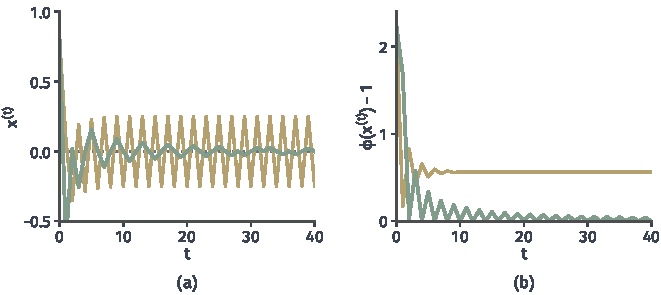
\includegraphics[width=112mm]{figures/05-optimization/07-multiple-criteria-and-nested-optimization/matplotlib/minimax-subgradient-worst/figure.pdf}
 \caption{精确响应加次梯度步，$\phi(x)=(\lvert x\rvert+1)^2$，起点$0.8$。黄线是固定步长$0.2$，绿线是递减步长$0.4/(t+1)$。(a)迭代点：黄线进入$\pm\frac14$的循环，绿线逐渐收敛到最优解$0$。(b)目标差：黄线停在$0.5625$，绿线继续下降。}
 \label{fig:minimax-subgradient-worst}
\end{BookInlineFigure}

这是第~\ref{chap:nonsmooth-composite-optimization}章次梯度法的典型行为，$\phi$是凸函数时那里的结论可以直接使用：有界次梯度下，步长取固定值$R/(G_{\mathrm{b}}\sqrt{T})$时平均点的目标差不超过$RG_{\mathrm{b}}/\sqrt{T}$，其中$R$是起点到解的距离上界，$G_{\mathrm{b}}$是次梯度范数上界。要让误差继续减小，步长必须递减。

\paragraph{局部极大不能代替全局最坏响应}
定理~\ref{thm:minimax-danskin}要的是全局最优响应。内层不凹时，内层算法通常只能找到局部极大点。看下面的函数，$Y=[-2,2]$：
\begin{equation}
 f(x,y)=\frac12x^2+xy+y^2-\frac14y^4.
 \label{eq:minimax-nonconcave}
\end{equation}

固定$x=1$，令$\partial_yf=1+2y-y^3=0$。因式分解得到
\[
 (y+1)(y^2-y-1)=0,
\]
三个根是$y=-1$，$y=\frac{1+\sqrt5}{2}\approx1.618$，$y=\frac{1-\sqrt5}{2}\approx-0.618$。计算得到
\[
 f(1,-1)=0.25,\qquad f(1,1.618)\approx3.023,\qquad f(1,-0.618)\approx0.227.
\]
$y=-1$是局部极大，$y=1.618$是全局极大，$y=-0.618$是局部极小，见图~\ref{fig:minimax-local-response}(a)。

\begin{BookInlineFigure}
 \centering
 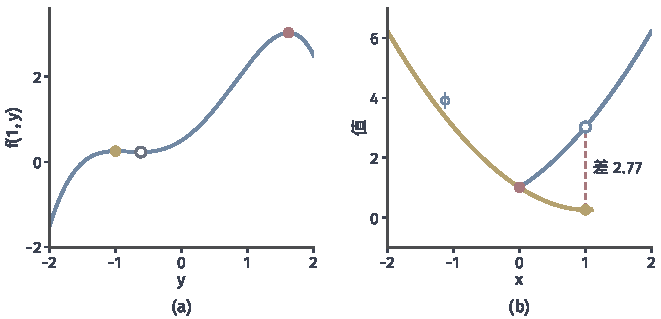
\includegraphics[width=112mm]{figures/05-optimization/07-multiple-criteria-and-nested-optimization/matplotlib/minimax-local-response/figure.pdf}
 \caption{内层不凹的例子，$f=\frac12x^2+xy+y^2-\frac14y^4$，$Y=[-2,2]$。(a)$x=1$时的内层函数：黄点是局部极大，红点是全局极大，空心点是局部极小。(b)蓝线是真实的$\phi$，红点是外层最优解；黄线是沿局部极大分支算得的值。$x=1$处两者相差$2.77$，局部分支到$x\approx1.089$处消失。}
 \label{fig:minimax-local-response}
\end{BookInlineFigure}

假设内层算法从$y<-0.618$的地方起步，它会收敛到$y=-1$。这一步的代价极大：报告的最坏值是$0.25$，真实值是$3.023$。更糟的是外层的方向，$\partial_xf=x+y$在这个响应处是
\[
 \partial_xf(1,-1)=0,
\]
看起来$x=1$已经驻定。而真实的导数是
\[
 \phi'(1)=1+1.618=2.618.
\]
图~\ref{fig:minimax-local-response}(b)中，黄线的局部分支一路下降，到$x=1$处还很低，蓝线的真实$\phi$却在升高。外层最优解其实是$x=0$，$\phi(0)=1$；局部分支报告的$0.25$甚至低于真正的最优值。

内层关于$\bm{y}$凹时，这个问题不存在，因为凹函数在凸集上的局部极大就是全局极大。否则，一个响应的“最优”只是相对于找到它的算法而言，后面报告结果时必须说明这一点。

\subsection{近似响应}
\label{sec:minimax-approx-response}

实际计算很少精确解内层，算到什么程度够用？先定义内层误差。

固定$\bm{x}$，对候选响应$\tilde{\bm{y}}\in\bm{Y}$，称
\begin{equation}
 \varepsilon=\phi(\bm{x})-f(\bm{x},\tilde{\bm{y}})\geq0
 \label{eq:minimax-inner-gap}
\end{equation}
为内层间隙。用它衡量比用$\bm{y}$的距离更合适，因为外层真正关心的是最坏值差多少。要把间隙转成外层梯度的误差，需要一座桥，这座桥就是强凹性：顶部越尖，间隙小就越能说明位置近，如同碗越陡，高度差小，水平距离就越小。

下面的条件贯穿本节。设$\bm{Y}$闭凸；$f$的梯度在$\bm{X}\times\bm{Y}$上$L$-Lipschitz；对每个$\bm{x}$，$f(\bm{x},\cdot)$在$\bm{Y}$上$\mu$强凹，$\mu>0$，记$\kappa=L/\mu$。

\begin{theorem}[内层间隙到外层梯度的传递]
\label{thm:minimax-inexact-gradient}
在上述条件下，内层响应唯一，记为$\bm{y}^\star(\bm{x})$。对任意$\tilde{\bm{y}}\in\bm{Y}$，
\begin{equation}
 \lVert\tilde{\bm{y}}-\bm{y}^\star(\bm{x})\rVert_2\leq\sqrt{\frac{2\varepsilon}{\mu}}.
 \label{eq:minimax-distance}
\end{equation}
进一步，
\begin{equation}
 \bigl\lVert\nabla_{\bm{x}}f(\bm{x},\tilde{\bm{y}})-\nabla_{\bm{x}}f(\bm{x},\bm{y}^\star(\bm{x}))\bigr\rVert_2\leq L\sqrt{\frac{2\varepsilon}{\mu}}.
 \label{eq:minimax-gradient-error}
\end{equation}
\end{theorem}

\begin{proof}
强凹函数在闭凸集上的最大点存在且唯一，记$\bm{y}^\star=\bm{y}^\star(\bm{x})$。最优性给出
\[
 \langle\nabla_{\bm{y}}f(\bm{x},\bm{y}^\star),\tilde{\bm{y}}-\bm{y}^\star\rangle\leq0.
\]
由$\mu$强凹的二次上界，
\[
 f(\bm{x},\tilde{\bm{y}})\leq f(\bm{x},\bm{y}^\star)+\langle\nabla_{\bm{y}}f(\bm{x},\bm{y}^\star),\tilde{\bm{y}}-\bm{y}^\star\rangle-\frac{\mu}{2}\lVert\tilde{\bm{y}}-\bm{y}^\star\rVert_2^2.
\]
把前一式代入，得到
\[
 f(\bm{x},\tilde{\bm{y}})\leq\phi(\bm{x})-\frac{\mu}{2}\lVert\tilde{\bm{y}}-\bm{y}^\star\rVert_2^2.
\]
移项就是式~\eqref{eq:minimax-distance}。再用$\nabla f$的Lipschitz性，就得到式~\eqref{eq:minimax-gradient-error}。
\end{proof}

用$f=-\frac12x^2+2xy-\frac12y^2$在$x=1$处核对，$\mu=1$，$y^\star=2$。取$\tilde{y}=1$，内层值和最坏值分别是
\[
 f(1,1)=1,\qquad\phi(1)=\frac32,
\]
所以$\varepsilon=\frac12$。式~\eqref{eq:minimax-distance}的右端是$1$，真实距离也是$1$，等号成立，因为这个内层函数恰好是二次的。

外层偏导数$\partial_xf=-1+2y$在$\tilde{y}=1$处是$1$，真实导数是$3$，误差是$2$，见图~\ref{fig:minimax-approx-response}。式~\eqref{eq:minimax-gradient-error}用$L=3$给出的上界是$3$，真实误差不超过它。这里交叉项的系数是$2$，把$L$换成$\partial_xf$对$y$的Lipschitz常数$2$，上界就是$2$，恰好等于真实误差。

\begin{BookInlineFigure}
 \centering
 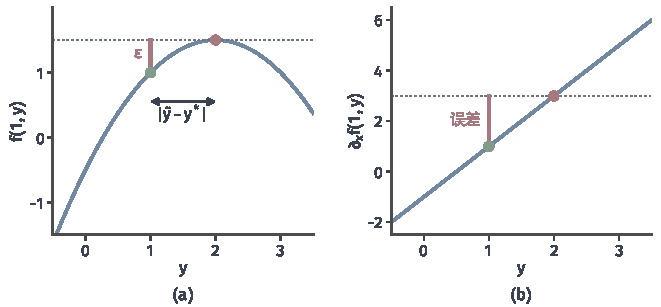
\includegraphics[width=112mm]{figures/05-optimization/07-multiple-criteria-and-nested-optimization/matplotlib/minimax-approx-response/figure.pdf}
 \caption{$f=-\frac12x^2+2xy-\frac12y^2$在$x=1$处。(a)内层函数，红点是最优响应，绿点是候选响应$\tilde{y}=1$，红线是内层间隙$\varepsilon=\frac12$，双箭头是响应距离。(b)外层偏导数关于$y$的直线，红点是真实导数$3$，绿点是候选给出的$1$，红线是误差。}
 \label{fig:minimax-approx-response}
\end{BookInlineFigure}

\paragraph{误差怎样影响外层}
梯度带误差时，外层下降还成立吗？先要知道$\phi$够光滑。下面的引理说明响应随$\bm{x}$平稳移动，从而$\phi$可微且梯度Lipschitz。这里不需要$\bm{Y}$紧。

\begin{lemma}[响应的稳定性与$\phi$的光滑性]
\label{lem:minimax-response-lipschitz}
在上述条件下，设$\bm{X}=\mathbb{R}^n$。则$\bm{y}^\star(\cdot)$是$\kappa$-Lipschitz的，$\phi$可微，梯度仍由式~\eqref{eq:minimax-danskin-gradient}的表达式给出，并且$\nabla\phi$是$L_\phi$-Lipschitz的，其中
\begin{equation}
 L_\phi=L(1+\kappa).
 \label{eq:minimax-phi-smooth}
\end{equation}
\end{lemma}

\begin{proof}
记$\bm{y}_1=\bm{y}^\star(\bm{x}_1)$，$\bm{y}_2=\bm{y}^\star(\bm{x}_2)$。两个最优性条件给出
\[
 \langle\nabla_{\bm{y}}f(\bm{x}_1,\bm{y}_1),\bm{y}_2-\bm{y}_1\rangle\leq0,\qquad\langle\nabla_{\bm{y}}f(\bm{x}_2,\bm{y}_2),\bm{y}_1-\bm{y}_2\rangle\leq0.
\]
$f(\bm{x}_2,\cdot)$的$\mu$强凹性给出
\[
 \mu\lVert\bm{y}_1-\bm{y}_2\rVert_2^2\leq\langle\nabla_{\bm{y}}f(\bm{x}_2,\bm{y}_2)-\nabla_{\bm{y}}f(\bm{x}_2,\bm{y}_1),\bm{y}_1-\bm{y}_2\rangle.
\]

右端含$\nabla_{\bm{y}}f(\bm{x}_2,\bm{y}_2)$的项由第二个最优性条件非正，可以丢掉，于是
\[
 \mu\lVert\bm{y}_1-\bm{y}_2\rVert_2^2\leq-\langle\nabla_{\bm{y}}f(\bm{x}_2,\bm{y}_1),\bm{y}_1-\bm{y}_2\rangle.
\]
在内积中加减$\nabla_{\bm{y}}f(\bm{x}_1,\bm{y}_1)$，并用第一个最优性条件丢掉一项，得到
\[
 \mu\lVert\bm{y}_1-\bm{y}_2\rVert_2^2\leq\langle\nabla_{\bm{y}}f(\bm{x}_1,\bm{y}_1)-\nabla_{\bm{y}}f(\bm{x}_2,\bm{y}_1),\bm{y}_1-\bm{y}_2\rangle.
\]
由Cauchy--Schwarz不等式和Lipschitz条件，得到
\[
 \lVert\bm{y}_1-\bm{y}_2\rVert_2\leq\kappa\lVert\bm{x}_1-\bm{x}_2\rVert_2.
\]

再证可微。任取$\bm{x}$和$\bm{d}$，记$\bm{y}=\bm{y}^\star(\bm{x})$，$\bm{y}_{\bm{d}}=\bm{y}^\star(\bm{x}+\bm{d})$，$\bm{g}=\nabla_{\bm{x}}f(\bm{x},\bm{y})$。用$\bm{y}$在$\bm{x}+\bm{d}$处的值作下界，并由光滑性，
\[
 \phi(\bm{x}+\bm{d})-\phi(\bm{x})\geq f(\bm{x}+\bm{d},\bm{y})-f(\bm{x},\bm{y})\geq\langle\bm{g},\bm{d}\rangle-\frac{L}{2}\lVert\bm{d}\rVert_2^2.
\]

用$\bm{y}_{\bm{d}}$作上界，同样由光滑性和响应的Lipschitz性，
\[
 \begin{aligned}
 \phi(\bm{x}+\bm{d})-\phi(\bm{x})&\leq f(\bm{x}+\bm{d},\bm{y}_{\bm{d}})-f(\bm{x},\bm{y}_{\bm{d}})\\
 &\leq\langle\nabla_{\bm{x}}f(\bm{x},\bm{y}_{\bm{d}}),\bm{d}\rangle+\frac{L}{2}\lVert\bm{d}\rVert_2^2\\
 &\leq\langle\bm{g},\bm{d}\rangle+L\kappa\lVert\bm{d}\rVert_2^2+\frac{L}{2}\lVert\bm{d}\rVert_2^2.
 \end{aligned}
\]
上下夹逼，得到$\phi$可微且梯度为$\bm{g}$。

最后，由梯度公式和响应的Lipschitz性，
\[
 \lVert\nabla\phi(\bm{x}_1)-\nabla\phi(\bm{x}_2)\rVert_2\leq L\lVert\bm{x}_1-\bm{x}_2\rVert_2+L\lVert\bm{y}_1-\bm{y}_2\rVert_2\leq L(1+\kappa)\lVert\bm{x}_1-\bm{x}_2\rVert_2.
\]
\end{proof}

式~\eqref{eq:minimax-phi-smooth}说明，$\phi$的光滑常数可能比$f$大$\kappa$倍。原因是响应会跟着$\bm{x}$动，$\kappa$越大响应动得越快，外层看到的函数越弯。

\begin{theorem}[带内层误差的外层下降]
\label{thm:minimax-inexact-descent}
在引理~\ref{lem:minimax-response-lipschitz}的条件下，设$\phi$有下界$\phi_{\inf}$，外层迭代$\bm{x}^{(t+1)}=\bm{x}^{(t)}-\alpha\bm{g}^{(t)}$，其中$0<\alpha\leq1/L_\phi$，$\bm{g}^{(t)}$与$\nabla\phi(\bm{x}^{(t)})$之差的范数不超过$\delta$。则
\begin{equation}
 \min_{0\leq t<T}\lVert\nabla\phi(\bm{x}^{(t)})\rVert_2^2\leq\frac{2(\phi(\bm{x}^{(0)})-\phi_{\inf})}{\alpha T}+\delta^2.
 \label{eq:minimax-inexact-descent}
\end{equation}
\end{theorem}

\begin{proof}
记$\bm{x}=\bm{x}^{(t)}$，$\bm{g}=\bm{g}^{(t)}$，$\bm{e}=\bm{g}-\nabla\phi(\bm{x})$。由$L_\phi$-光滑的下降引理和$\alpha L_\phi\leq1$，
\[
 \phi(\bm{x}^{(t+1)})\leq\phi(\bm{x})-\alpha\langle\nabla\phi(\bm{x}),\bm{g}\rangle+\frac{\alpha}{2}\lVert\bm{g}\rVert_2^2.
\]
对任意向量$\bm{a},\bm{b}$有恒等式
\[
 -\langle\bm{a},\bm{b}\rangle+\frac12\lVert\bm{b}\rVert_2^2=\frac12\lVert\bm{b}-\bm{a}\rVert_2^2-\frac12\lVert\bm{a}\rVert_2^2.
\]
取$\bm{a}=\nabla\phi(\bm{x})$，$\bm{b}=\bm{g}$，得到
\[
 \phi(\bm{x}^{(t+1)})\leq\phi(\bm{x})-\frac{\alpha}{2}\lVert\nabla\phi(\bm{x})\rVert_2^2+\frac{\alpha}{2}\lVert\bm{e}\rVert_2^2.
\]
对$t=0,\ldots,T-1$求和，用$\phi(\bm{x}^{(T)})\geq\phi_{\inf}$和$\lVert\bm{e}\rVert_2\leq\delta$，再除以$\alpha T/2$，左端的平均不小于最小值，即得结论。
\end{proof}

式~\eqref{eq:minimax-inexact-descent}有两项：第一项随$T$下降，第二项是内层误差留下的平台。要让外层梯度小到$\epsilon$，内层误差$\delta$也要到$\epsilon$量级。结合式~\eqref{eq:minimax-gradient-error}，这要求内层间隙满足$L\sqrt{2\varepsilon/\mu}\lesssim\epsilon$，即$\varepsilon$是$\mu\epsilon^2/L^2$量级。

\paragraph{计算过程}
内层用$K$步投影梯度上升，并从上一轮的响应出发，比从头开始省事，因为$\bm{x}$变化不大时响应也变化不大。仍用$f=-\frac12x^2+2xy-\frac12y^2$。

\needspace{6\baselineskip}
\paragraph{变量}
\begin{itemize}
 \item $x^{(t)}$：外层变量；
 \item $y^{(t)}$：第$t$轮内层结束后的近似响应；
 \item $K$：每轮内层步数；$\beta$：内层步长；$\alpha$：外层步长。
\end{itemize}

\paragraph{初始化}
取$x^{(0)}$和$y^{(-1)}$。例中$x^{(0)}=1$，$y^{(-1)}=0$，$K=2$，$\beta=\frac12$，$\alpha=\frac16$。内层的曲率是$1$，步长$\beta=\frac12$不超过曲率的倒数。

\needspace{6\baselineskip}
\paragraph{每轮更新}
\begin{enumerate}
 \item 从$y=y^{(t-1)}$出发做$K$次内层更新$y\leftarrow P_Y(y+\beta\partial_yf(x^{(t)},y))$，得$y^{(t)}$。例中$\partial_yf=2x-y$，第一轮
 \[
  y:\ 0\to0+\frac12\cdot2=1\to1+\frac12\cdot1=1.5,\qquad y^{(0)}=1.5.
 \]
 \item 用当前响应计算外层偏导数$g^{(t)}=\partial_xf(x^{(t)},y^{(t)})$。例中第一轮
 \[
  g^{(0)}=-1+2\cdot1.5=2.
 \]
 \item 更新外层$x^{(t+1)}=x^{(t)}-\alpha g^{(t)}$。例中第一轮
 \[
  x^{(1)}=1-\frac26=\frac23.
 \]
\end{enumerate}

第二轮内层从$y=1.5$出发，目标$2x^{(1)}=\frac43$，两步给出
\[
 y:\ 1.5\to1.41667\to1.375,\qquad y^{(1)}=1.375.
\]
外层偏导数是$g^{(1)}=-\frac23+2.75\approx2.0833$，所以$x^{(2)}\approx0.3194$。真实导数$3x^{(1)}=2$，这一轮的误差约为$0.083$。

第一轮的真实导数是$3$，误差是$1$；第二轮暖启动之后，误差降到$0.083$。迭代继续下去，到设定的外层梯度精度为止。这里用$\lvert g^{(t)}\rvert$作判据时要记住，它自身带有内层误差。

\paragraph{一般非凹内层}
上面的传递依赖强凹性。没有强凹性时，$\nabla_{\bm{y}}f$很小不说明响应接近最优。式~\eqref{eq:minimax-nonconcave}中$(x,y)=(1,-1)$的内层梯度严格为零，内层间隙却是$2.77$。此时只从$\tilde{\bm{y}}$算出的值只是$\phi(\bm{x})$的下界，真实误差不可知，外层停止时必须说明实际使用的响应证据：用了什么内层算法、多少起点、最后的残差，而不能把$\nabla_{\bm{y}}f\approx\bm{0}$说成“内层已解”。

\section{下降—上升方法}
\label{sec:minimax-gda}

内层响应法每轮都要解一个优化问题，代价不小。能不能每轮只算一次两侧的梯度，让$\bm{x}$走一小步下山，同时让$\bm{y}$走一小步上山？本节研究这个最便宜的做法，它在什么情况下行得通，在什么情况下行不通。

\paragraph{主要思想}
设$\bm{X},\bm{Y}$是闭凸集，$f$可微。不再要求内层解到最优，而是让$\bm{y}$只沿内层目标的梯度走一步，$\bm{x}$沿外层方向走一步。这样的方法称为\term{梯度下降—上升}（gradient descent--ascent，GDA）。

两个偏梯度都在旧点计算，称为同时更新：
\begin{equation}
 \begin{aligned}
 \bm{x}^{(t+1)}&=P_{\bm{X}}\bigl(\bm{x}^{(t)}-\alpha\nabla_{\bm{x}}f(\bm{x}^{(t)},\bm{y}^{(t)})\bigr),\\
 \bm{y}^{(t+1)}&=P_{\bm{Y}}\bigl(\bm{y}^{(t)}+\beta\nabla_{\bm{y}}f(\bm{x}^{(t)},\bm{y}^{(t)})\bigr).
 \end{aligned}
 \label{eq:minimax-gda-sim}
\end{equation}

先更新$\bm{x}$，再用新的$\bm{x}$算$\bm{y}$的梯度，称为先后更新：
\begin{equation}
 \begin{aligned}
 \bm{x}^{(t+1)}&=P_{\bm{X}}\bigl(\bm{x}^{(t)}-\alpha\nabla_{\bm{x}}f(\bm{x}^{(t)},\bm{y}^{(t)})\bigr),\\
 \bm{y}^{(t+1)}&=P_{\bm{Y}}\bigl(\bm{y}^{(t)}+\beta\nabla_{\bm{y}}f(\bm{x}^{(t+1)},\bm{y}^{(t)})\bigr).
 \end{aligned}
 \label{eq:minimax-gda-alt}
\end{equation}

两式只有第二行里$\bm{x}$的上标不同，却是不同的递推，下面的例子里轨迹的性质也不同。比较时必须说明用的是哪一种。

\paragraph{计算过程}
用$f(x,y)=xy$，$X=Y=\mathbb{R}$，唯一鞍点是原点。

\needspace{6\baselineskip}
\paragraph{变量}
\begin{itemize}
 \item $x^{(t)},y^{(t)}$：两组变量；
 \item $\alpha,\beta>0$：两侧步长。
\end{itemize}

\paragraph{初始化}
取$(x^{(0)},y^{(0)})$。例中$(x^{(0)},y^{(0)})=(1,0)$，$\alpha=\beta=\frac12$。

\needspace{6\baselineskip}
\paragraph{每轮更新}
\begin{enumerate}
 \item 计算两个偏导数。例中$\partial_xf=y$，$\partial_yf=x$。
 \item 按式~\eqref{eq:minimax-gda-sim}或式~\eqref{eq:minimax-gda-alt}更新。例中同时更新的第一轮
 \[
  x^{(1)}=1-\frac12\cdot0=1,\qquad y^{(1)}=0+\frac12\cdot1=\frac12.
 \]
 第二轮、第三轮分别得到
 \[
  (x^{(2)},y^{(2)})=(0.75,1),\qquad(x^{(3)},y^{(3)})=(0.25,1.375).
 \]
 \item 先后更新的第一轮结果相同，因为$y^{(0)}=0$时$x$不动。第二轮和第三轮分别是
 \[
  (x^{(2)},y^{(2)})=(0.75,0.875),\qquad(x^{(3)},y^{(3)})=(0.3125,1.03125).
 \]
\end{enumerate}

通常的结束条件是步数达到上限，或残差小于容差。例中距离鞍点的平方，同时更新依次为$1,1.25,1.5625,1.953$，每轮乘以$1.25$；先后更新依次为$1,1.25,1.3281,1.161$，有界地上下波动。最终两种更新都没有接近鞍点。下一小节解释原因。

\subsection{旋转现象}
\label{sec:minimax-rotation}

把同时更新用矩阵写出来，记$\bm{z}=(x,y)^\top$，式~\eqref{eq:minimax-gda-sim}成为
\begin{equation}
 \bm{z}^{(t+1)}=\begin{pmatrix}1&-\alpha\\\alpha&1\end{pmatrix}\bm{z}^{(t)}.
 \label{eq:minimax-gda-matrix}
\end{equation}

这个矩阵是一个旋转矩阵乘以$\sqrt{1+\alpha^2}$。两列互相正交，长度都是$\sqrt{1+\alpha^2}$，所以
\begin{equation}
 \lVert\bm{z}^{(t+1)}\rVert_2^2=(1+\alpha^2)\lVert\bm{z}^{(t)}\rVert_2^2.
 \label{eq:minimax-gda-growth}
\end{equation}

对任何固定的$\alpha>0$，距离都按几何级数增长。$\alpha=\frac12$时每轮乘以$1.25$，与上面的数字一致。步长取得再小，也只是增长得慢，不会变成收缩。

几何上，迭代方向是$(-y,x)$，它和位置向量$(x,y)$处处垂直，也就是沿着以原点为圆心的圆的切线方向。沿切线走一小段，总是落到更大的圆上。这像绕着一个圆运动的人每走一步都沿当前切线走直线，路线不是回到原圆，而是向外盘旋。连续时间的方程$\dot{\bm{z}}=(-y,x)$恰好沿圆运动，半径不变；离散化把这个“恰好不靠近”的运动变成了发散。

先后更新的矩阵是
\[
 \begin{pmatrix}1&-\alpha\\\alpha&1-\alpha^2\end{pmatrix},
\]
行列式是$1$，迹是$2-\alpha^2$。$0<\alpha<2$时迹的绝对值小于$2$，两个特征值是模为$1$的共轭复数，迭代既不发散也不收敛。

这一点可以用一个守恒量看得更清楚。令$Q=x^2+y^2-\alpha xy$，记$x^{+}=x-\alpha y$，$y^{+}=y+\alpha x^{+}$。先处理含$y^{+}$的两项：
\[
 (y^{+})^2-\alpha x^{+}y^{+}=y^{+}(y^{+}-\alpha x^{+})=y^{+}y=y^2+\alpha x^{+}y.
\]
再处理剩下的项：
\[
 (x^{+})^2+\alpha x^{+}y=x^{+}(x^{+}+\alpha y)=x^{+}x=x^2-\alpha xy.
\]
两式相加，得到
\[
 (x^{+})^2+(y^{+})^2-\alpha x^{+}y^{+}=x^2+y^2-\alpha xy,
\]
所以$Q$沿迭代不变。$0<\alpha<2$时$Q$是正定二次型，迭代点永远留在同一个椭圆上，既跑不掉也到不了中心。图~\ref{fig:minimax-gda-rotation}(a)(b)画出了两种轨迹。

\begin{BookInlineFigure}
 \centering
 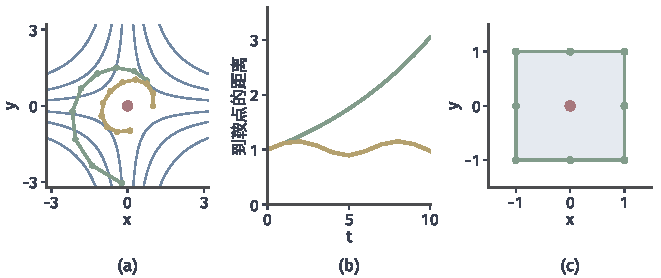
\includegraphics[width=112mm]{figures/05-optimization/07-multiple-criteria-and-nested-optimization/matplotlib/minimax-gda-rotation/figure.pdf}
 \caption{$f=xy$上的下降—上升，蓝线是等高线，红点是鞍点。(a)$\alpha=\frac12$，起点$(1,0)$，$10$步：绿色是同时更新，向外盘旋；黄色是先后更新，留在椭圆上。(b)两种更新到鞍点的距离。(c)盒子$[-1,1]^2$上的投影同时更新，$\alpha=1$，从$(1,0)$出发，$8$步回到起点。}
 \label{fig:minimax-gda-rotation}
\end{BookInlineFigure}

\paragraph{加上约束也不收敛}
把迭代限制在盒子里能防止发散，却不能让它停在鞍点。取$X=Y=[-1,1]$，$\alpha=\beta=1$，从$(1,0)$出发做投影同时更新，投影就是逐分量截断到$[-1,1]$。第一步$x=1-0=1$，$y=0+1=1$；第二步$x=1-1=0$，$y=1+1=2$，截断成$1$。继续算下去，得到
\[
 \begin{aligned}
 (1,0)&\to(1,1)\to(0,1)\to(-1,1)\to(-1,0)\\
 &\to(-1,-1)\to(0,-1)\to(1,-1)\to(1,0).
 \end{aligned}
\]

八步之后回到起点，见图~\ref{fig:minimax-gda-rotation}(c)。由式~\eqref{eq:minimax-box-gap}，循环上的间隙$\lvert x\rvert+\lvert y\rvert$取$1$或$2$，永远不小于$1$。定理~\ref{thm:minimax-theorem}的条件全部满足，鞍点存在，算法却找不到它。存在性定理回答解在不在，不回答某个算法能否到达。

\paragraph{只看一侧的数不足以判断}
图~\ref{fig:minimax-gda-monitor}(a)是同时更新过程中$f(x^{(t)},y^{(t)})$的值。从$t=2$到$t=5$，它从$0.75$一路降到$-1.52$。如果只看这条线，会以为外层目标在稳步下降，而图~\ref{fig:minimax-gda-monitor}(b)显示点正在远离解。$f$的值本来就该由一侧压低、另一侧抬高，它的升降不说明任何问题。

\begin{BookInlineFigure}
 \centering
 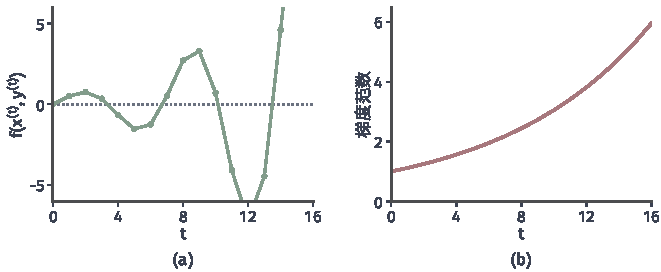
\includegraphics[width=112mm]{figures/05-optimization/07-multiple-criteria-and-nested-optimization/matplotlib/minimax-gda-monitor/figure.pdf}
 \caption{$f=xy$上同时更新的监控量，$\alpha=\frac12$，起点$(1,0)$。(a)绿线是代价$f$的值，在部分时段连续下降，又在更大的幅度上振荡。(b)红线是两侧梯度的范数$\lVert(y,-x)\rVert_2$，它等于到鞍点的距离，持续增长。}
 \label{fig:minimax-gda-monitor}
\end{BookInlineFigure}

反过来，梯度为零也说明不了稳定。对$f=xy$，原点两侧梯度都为零，而且原点就是解，迭代却从任何非零点开始都远离它，一旦有扰动也回不去。对$f=y^2-x^2$，原点两侧梯度也为零，但迭代$x^{+}=(1+2\alpha)x$，$y^{+}=(1+2\alpha)y$从原点附近往外推，原点又不是解。所以驻定只回答“这个点本身怎样”，不回答“迭代会不会留在它附近”，后者要看迭代映射的线性化。

\subsection{响应速度}
\label{sec:minimax-speed}

$f=xy$没有内层曲率，$\bm{y}$没有自己想去的位置。内层有强凹性时，$\bm{y}$就有一个目标$\bm{y}^\star(\bm{x})$，问题变成：$\bm{y}$能否跟上这个随$\bm{x}$移动的目标？

继续用$f=-\frac12x^2+2xy-\frac12y^2$，最优响应是$y=2x$，原点是顺序问题的解。令$\beta=r\alpha$，$r$是两侧步长之比。迭代$\bm{z}^{+}=(\bm{I}-\alpha\bm{J}_r)\bm{z}$的矩阵是
\begin{equation}
 \bm{J}_r=\begin{pmatrix}-1&2\\-2r&r\end{pmatrix}.
 \label{eq:minimax-timescale-matrix}
\end{equation}

$\bm{J}_r$的迹是$r-1$，行列式是$3r$。当$1<r<13$时，判别式$(r-1)^2-12r<0$，两个特征值是共轭复数$\lambda$，满足$\operatorname{Re}\lambda=\frac{r-1}{2}$，$\lvert\lambda\rvert^2=3r$。迭代的模平方是
\[
 \lvert1-\alpha\lambda\rvert^2=1-\alpha(r-1)+3r\alpha^2.
\]

这个量小于$1$，当且仅当
\begin{equation}
 0<\alpha<\frac{r-1}{3r}.
 \label{eq:minimax-timescale-stable}
\end{equation}

$r=1$时模平方是$1+3\alpha^2>1$，任何步长都发散。$r<1$时两个特征值的实部为负，$\lvert1-\alpha\lambda\rvert>1$，同样发散。$r=4$时条件是$\alpha<\frac14$，例如$\alpha=0.1$时模平方是$0.82$。两种选择用同样的$\alpha$，差别只在$y$走得快不快，见图~\ref{fig:minimax-timescale}。

\begin{BookInlineFigure}
 \centering
 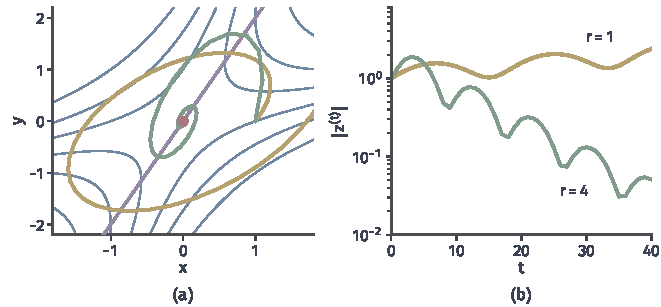
\includegraphics[width=112mm]{figures/05-optimization/07-multiple-criteria-and-nested-optimization/matplotlib/minimax-timescale/figure.pdf}
 \caption{$f=-\frac12x^2+2xy-\frac12y^2$上的同时更新，$\alpha=0.1$，起点$(1,0)$，$40$步。蓝线是等高线，紫线是最优响应$y=2x$，红点是解。黄线$r=1$，两侧同速，$y$跟不上$x$，轨迹向外盘旋。绿线$r=4$，$y$走得快，轨迹贴着紫线向解收敛。(b)到解的距离。}
 \label{fig:minimax-timescale}
\end{BookInlineFigure}

$r$的门槛来自$f$的结构。$\partial_x^2f=-1$是外层变量的负曲率，$\partial_y^2f=-1$是内层变量提供的强凹性。外层独自运动时是往外推的，只有$y$足够快地跟上$y=2x$，外层才看得到$\phi''=3>0$的正曲率。$y$落后时，外层感受到的是$f$在旧$y$上的负曲率，于是被推开。

\paragraph{跟踪误差的递推}
一般情形可以用跟踪误差来刻画这种竞赛。沿用第~\ref{sec:minimax-approx-response}节的条件，记跟踪误差为
\begin{equation}
 e_t=\lVert\bm{y}^{(t)}-\bm{y}^\star(\bm{x}^{(t)})\rVert_2.
 \label{eq:minimax-tracking-error}
\end{equation}

第~\ref{chap:feasible-iterations}章证明过：$\mu$强凸、$L$-光滑的函数上，步长为$1/L$的投影梯度法把到解的距离至少缩小到$\rho=\sqrt{1-\mu/L}$倍。把它用到凸函数$-f(\bm{x},\cdot)$上。

\begin{lemma}[跟踪误差的递推]
\label{lem:minimax-tracking}
设$\bm{x}^{(t+1)}$已经算出，从$\bm{y}^{(t)}$出发在$f(\bm{x}^{(t+1)},\cdot)$上做$K$步步长$1/L$的投影梯度上升，得到$\bm{y}^{(t+1)}$。则
\begin{equation}
 e_{t+1}\leq\rho^{K}\bigl(e_t+\kappa\lVert\bm{x}^{(t+1)}-\bm{x}^{(t)}\rVert_2\bigr).
 \label{eq:minimax-tracking}
\end{equation}
\end{lemma}

\begin{proof}
$K$步投影梯度上升的收缩给出
\[
 e_{t+1}\leq\rho^K\lVert\bm{y}^{(t)}-\bm{y}^\star(\bm{x}^{(t+1)})\rVert_2.
\]
用三角不等式，并由引理~\ref{lem:minimax-response-lipschitz}的$\kappa$-Lipschitz性，
\[
 \lVert\bm{y}^{(t)}-\bm{y}^\star(\bm{x}^{(t+1)})\rVert_2\leq e_t+\kappa\lVert\bm{x}^{(t+1)}-\bm{x}^{(t)}\rVert_2.
\]
两式合起来即得。
\end{proof}

式~\eqref{eq:minimax-tracking}里，$\rho^K$是内层追赶的速度，$\kappa\lVert\bm{x}^{(t+1)}-\bm{x}^{(t)}\rVert_2$是目标跑开的距离。要跟得上，有两种办法：增加$K$，或者减小外层步长。

取$K=1$，看外层步长要小到什么程度。设每步外层移动量是$\alpha\lVert\bm{g}\rVert_2$，$\rho\approx1-\frac{1}{2\kappa}$。递推的稳态是
\[
 e_\infty\approx\frac{\kappa\alpha\lVert\bm{g}\rVert_2}{1-\rho}\approx2\kappa^2\alpha\lVert\bm{g}\rVert_2.
\]

外层梯度的误差约为$Le_\infty$。要让它不超过$\frac12\lVert\bm{g}\rVert_2$，需要$\alpha\lesssim\frac{1}{4\kappa^2L}$，也就是$\alpha/\beta$是$1/\kappa^2$量级。这个推算只是说明量级，不是证明。完整的结论要把式~\eqref{eq:minimax-tracking}和定理~\ref{thm:minimax-inexact-descent}放进同一个势函数，得到的是非凸—强凹问题上求$\phi$的$\epsilon$驻定点需要$O(\kappa^2/\epsilon^2)$量级的梯度读取。该证明篇幅较长，读者可查阅双时间尺度下降—上升的专门分析。

理论的步长是保守的。上例$L=3$，$\kappa=3$，上述量级给出的$\alpha$约为$\frac{1}{108}$，而取$\beta=\frac13$时由式~\eqref{eq:minimax-timescale-stable}可算出实际的稳定范围到$\alpha<\frac16$。保证覆盖的是一个函数类中最差的情形，这与第~\ref{chap:first-order-methods}章步长的保守取法一样。

\paragraph{非凸—非凹情形}
以上依赖强凹性带来的$\kappa$-Lipschitz响应。式~\eqref{eq:minimax-nonconcave}中最优响应在$x=0$处从$-\sqrt2$跳到$\sqrt2$，没有任何Lipschitz常数，内层再快也不能平稳地跟踪。此时必须分别说明三件事：用的是什么步长组合，内层响应求到了什么程度，所报告的驻定概念是什么，第~\ref{sec:minimax-evaluation}节回到这些问题。一般非凸—非凹问题上，下降—上升可能循环，也可能发散，没有与上面同类的保证。

\section{校正方向}
\label{sec:minimax-correction}

上一节的失败发生在凸凹问题上，而且鞍点存在。所以问题不在问题本身，在迭代格式。本节先把鞍点条件写成统一的形式，看清旋转是从哪里来的，再修改迭代，用另一处的方向校正当前一步。

\paragraph{变分不等式形式}
把两组变量合并，记$\bm{z}=(\bm{x},\bm{y})$，$\bm{Z}=\bm{X}\times\bm{Y}$，定义
\begin{equation}
 \bm{F}(\bm{z})=\begin{pmatrix}\nabla_{\bm{x}}f(\bm{x},\bm{y})\\-\nabla_{\bm{y}}f(\bm{x},\bm{y})\end{pmatrix}.
 \label{eq:minimax-operator}
\end{equation}

两侧步长相同时，同时更新就是
\[
 \bm{z}^{+}=P_{\bm{Z}}\bigl(\bm{z}-\alpha\bm{F}(\bm{z})\bigr).
\]

它和投影梯度法外形一样，但$\bm{F}$一般不是任何函数的梯度。鞍点条件也能用$\bm{F}$写出来，这个写法就是第~\ref{chap:constrained-optimality}章见过的变分不等式。

\begin{theorem}[鞍点的变分不等式刻画]
\label{thm:minimax-vi}
设$\bm{X},\bm{Y}$非空闭凸，$f$在含$\bm{Z}$的开集上可微，关于$\bm{x}$凸，关于$\bm{y}$凹。则$\bm{z}^\star\in\bm{Z}$是全局鞍点，当且仅当
\begin{equation}
 \langle\bm{F}(\bm{z}^\star),\bm{z}-\bm{z}^\star\rangle\geq0\qquad\text{对所有}\ \bm{z}\in\bm{Z}.
 \label{eq:minimax-vi}
\end{equation}
\end{theorem}

\begin{proof}
记$\bm{z}^\star=(\bm{x}^\star,\bm{y}^\star)$。设它是鞍点。$\bm{x}^\star$在凸集$\bm{X}$上最小化可微凸函数$f(\cdot,\bm{y}^\star)$，一阶条件给出
\[
 \langle\nabla_{\bm{x}}f(\bm{z}^\star),\bm{x}-\bm{x}^\star\rangle\geq0.
\]
$\bm{y}^\star$在$\bm{Y}$上最大化凹函数$f(\bm{x}^\star,\cdot)$，一阶条件给出
\[
 \langle-\nabla_{\bm{y}}f(\bm{z}^\star),\bm{y}-\bm{y}^\star\rangle\geq0.
\]
两式相加即为式~\eqref{eq:minimax-vi}。

反过来，在式~\eqref{eq:minimax-vi}中取$\bm{z}=(\bm{x},\bm{y}^\star)$，得到上面第一式，由凸性，$\bm{x}^\star$是$f(\cdot,\bm{y}^\star)$的全局最小点。取$\bm{z}=(\bm{x}^\star,\bm{y})$，得到第二式，由凹性，$\bm{y}^\star$是$f(\bm{x}^\star,\cdot)$的全局最大点。这就是式~\eqref{eq:minimax-saddle}。
\end{proof}

式~\eqref{eq:minimax-vi}的几何含义是，从$\bm{z}^\star$看向任何可行方向，它与$\bm{F}(\bm{z}^\star)$的夹角都不超过直角，见图~\ref{fig:minimax-vi-geometry}。

\begin{BookInlineFigure}
 \centering
 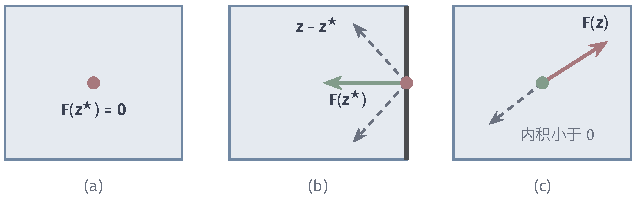
\includegraphics[width=107.7mm]{figures/05-optimization/07-multiple-criteria-and-nested-optimization/tikz/minimax-vi-geometry/figure.pdf}
 \caption{变分不等式的几何。浅蓝矩形是$\bm{Z}$。(a)解在内部时$\bm{F}(\bm{z}^\star)=\bm{0}$。(b)解在边界（深灰粗线）上时$\bm{F}(\bm{z}^\star)$指向内部，虚线表示的可行方向$\bm{z}-\bm{z}^\star$都与它成锐角。(c)绿点不是解，存在可行方向与红色的$\bm{F}(\bm{z})$内积为负。}
 \label{fig:minimax-vi-geometry}
\end{BookInlineFigure}

$\bm{F}$的性质由凸凹性决定。

\begin{lemma}[单调性]
\label{lem:minimax-monotone}
在定理~\ref{thm:minimax-vi}的条件下，$\bm{F}$是\term{单调算子}（monotone operator），即对任意$\bm{z}_1,\bm{z}_2\in\bm{Z}$，
\begin{equation}
 \langle\bm{F}(\bm{z}_1)-\bm{F}(\bm{z}_2),\bm{z}_1-\bm{z}_2\rangle\geq0.
 \label{eq:minimax-monotone}
\end{equation}
\end{lemma}

\begin{proof}
记$\bm{z}_i=(\bm{x}_i,\bm{y}_i)$。由$f(\cdot,\bm{y}_1)$和$f(\cdot,\bm{y}_2)$的凸性，
\[
 \begin{aligned}
 f(\bm{x}_2,\bm{y}_1)&\geq f(\bm{x}_1,\bm{y}_1)+\langle\nabla_{\bm{x}}f(\bm{z}_1),\bm{x}_2-\bm{x}_1\rangle,\\
 f(\bm{x}_1,\bm{y}_2)&\geq f(\bm{x}_2,\bm{y}_2)+\langle\nabla_{\bm{x}}f(\bm{z}_2),\bm{x}_1-\bm{x}_2\rangle.
 \end{aligned}
\]
由$f(\bm{x}_1,\cdot)$和$f(\bm{x}_2,\cdot)$的凹性，
\[
 \begin{aligned}
 f(\bm{x}_1,\bm{y}_2)&\leq f(\bm{x}_1,\bm{y}_1)+\langle\nabla_{\bm{y}}f(\bm{z}_1),\bm{y}_2-\bm{y}_1\rangle,\\
 f(\bm{x}_2,\bm{y}_1)&\leq f(\bm{x}_2,\bm{y}_2)+\langle\nabla_{\bm{y}}f(\bm{z}_2),\bm{y}_1-\bm{y}_2\rangle.
 \end{aligned}
\]
把四个不等式相加，函数值全部相消，整理即得式~\eqref{eq:minimax-monotone}。
\end{proof}

单调是梯度单调的推广，$f$是凸函数时$\nabla f$单调。差别在于$\bm{F}$的Jacobian不对称。$f$二阶可微时，
\[
 \bm{J}=\begin{pmatrix}\nabla^2_{\bm{x}\bm{x}}f&\nabla^2_{\bm{x}\bm{y}}f\\-\nabla^2_{\bm{y}\bm{x}}f&-\nabla^2_{\bm{y}\bm{y}}f\end{pmatrix}.
\]

对角块由凸凹性是半正定的，贡献朝向解的收缩。非对角块反对称，贡献的是旋转，它对$\langle\bm{F}(\bm{z})-\bm{F}(\bm{z}'),\bm{z}-\bm{z}'\rangle$的贡献恰好是零。$f=xy$时对角块全是零，$\bm{J}$只剩反对称部分，所以$\langle\bm{F}(\bm{z}),\bm{z}\rangle=0$。单调性在这里只说明方向不朝外，并不提供任何朝向解的分量，这就是旋转现象的代数来源。

\paragraph{校正的想法}
旋转场里，当前点的方向用一整步就过时了，走到新位置时场已经转了角度。一个自然的修补是：先试探着走一步，读取试探点处的方向，再回到原来的位置，用这个方向走一步。下面的表把这个想法和几种看起来相近的技巧放在一起。

\begin{BookInlineTable}
 \centering
 \begin{tabular}{@{}lll@{}}
  \toprule
  技巧 & 改的是什么 & 对$f=xy$的效果\\
  \midrule
  重球动量 & 叠加上一步的位移 & 把切向位移加强，更快发散\\
  乘子法 & 改目标，加增广项后解内层 & 需要解子问题\\
  外梯度 & 方向取自预测点 & 收缩\\
  乐观梯度 & 用方向的差分校正 & 收缩\\
  \bottomrule
 \end{tabular}
 \caption{几种修改迭代或目标的办法。前两种不是校正方向。}
 \label{tab:minimax-correction-compare}
\end{BookInlineTable}

重球法是第~\ref{chap:first-order-methods}章的单目标加速，叠加的是位置差$\bm{z}^{(t)}-\bm{z}^{(t-1)}$。在$f=xy$上，上一步的位移本身就是切向的，叠加之后向外偏得更多。取$\alpha=0.2$，动量系数$0.5$，迭代的谱半径是$1.125$，比不加动量时的$1.020$还大。

第~\ref{chap:penalty-multiplier-methods}章的乘子法也交替更新原变量和乘子，但它在$\bm{x}$上解一个增广Lagrange子问题，增广项改变了目标。校正方向不改$f$，只改读取方向的位置，每轮仍只是读取几次方向。

\subsection{外梯度法}
\label{sec:minimax-extragradient}

\paragraph{主要思想}
\term{外梯度法}（extragradient method，EG）每轮读取两次方向\scite{korpelevich1976}。先从当前点走一个试探步，读取新方向，再回到当前点，用新方向完成校正：
\begin{equation}
 \begin{aligned}
 \tilde{\bm{z}}^{(t)}&=P_{\bm{Z}}\bigl(\bm{z}^{(t)}-\alpha\bm{F}(\bm{z}^{(t)})\bigr),\\
 \bm{z}^{(t+1)}&=P_{\bm{Z}}\bigl(\bm{z}^{(t)}-\alpha\bm{F}(\tilde{\bm{z}}^{(t)})\bigr).
 \end{aligned}
 \label{eq:minimax-eg}
\end{equation}

校正步的起点仍是$\bm{z}^{(t)}$，只是方向换成了试探点的方向。这和连续做两次普通梯度步不同，后者的第二步从$\tilde{\bm{z}}^{(t)}$出发。

为什么这样能收缩？看$f=xy$，$\bm{F}(x,y)=(y,-x)$。在图~\ref{fig:minimax-eg-step}中，从$\bm{z}$沿切线走到$\tilde{\bm{z}}$，那里的方向已经向内转过了一个角度。把这个方向拿回$\bm{z}$，迈出的一步就略微朝向圆内，抵消了切线外漂。

\begin{BookInlineFigure}
 \centering
 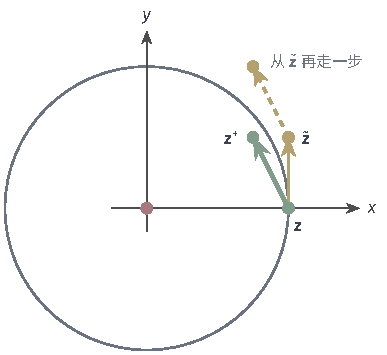
\includegraphics[width=65.6mm]{figures/05-optimization/07-multiple-criteria-and-nested-optimization/tikz/minimax-eg-step/figure.pdf}
 \caption{外梯度的一步，$f=xy$，$\alpha=\frac12$。灰色圆是过$\bm{z}=(1,0)$的等距圆，红点是鞍点。黄色实线箭头走到试探点$\tilde{\bm{z}}=(1,0.5)$，绿色箭头从$\bm{z}$沿试探点的方向走到$\bm{z}^{+}=(0.75,0.5)$，落在圆内。黄色虚线是从试探点再走一步普通梯度步，到$(0.75,1)$，落在圆外。}
 \label{fig:minimax-eg-step}
\end{BookInlineFigure}

代数上，把$\bm{F}(\bm{z})=\bm{A}\bm{z}$代入，$\bm{A}=\begin{pmatrix}0&1\\-1&0\end{pmatrix}$，得到
\[
 \bm{z}^{+}=\bm{z}-\alpha\bm{A}(\bm{z}-\alpha\bm{A}\bm{z})=\bigl(\bm{I}-\alpha\bm{A}+\alpha^2\bm{A}^2\bigr)\bm{z}.
\]

由于$\bm{A}^2=-\bm{I}$，上式成为$\bm{z}^{+}=(1-\alpha^2)\bm{z}-\alpha\bm{A}\bm{z}$。$\bm{z}$与$\bm{A}\bm{z}$正交，长度相同，所以
\begin{equation}
 \lVert\bm{z}^{+}\rVert_2^2=\bigl(1-\alpha^2+\alpha^4\bigr)\lVert\bm{z}\rVert_2^2.
 \label{eq:minimax-eg-contraction}
\end{equation}
$0<\alpha<1$时这个因子小于$1$。多读取的那一次方向，把式~\eqref{eq:minimax-gda-growth}里的$+\alpha^2$换成了$-\alpha^2$，这是二阶项的差别。

\paragraph{计算过程}
用$f=xy$，$X=Y=\mathbb{R}$，投影是恒等映射。

\needspace{6\baselineskip}
\paragraph{变量}
\begin{itemize}
 \item $\bm{z}^{(t)}=(x^{(t)},y^{(t)})$：当前点；
 \item $\tilde{\bm{z}}^{(t)}$：试探点；
 \item $\alpha>0$：步长。
\end{itemize}

\paragraph{初始化}
取$\bm{z}^{(0)}\in\bm{Z}$。例中$\bm{z}^{(0)}=(1,0)$，$\alpha=\frac12$，与上一节相同，便于比较。

\needspace{6\baselineskip}
\paragraph{每轮更新}
\begin{enumerate}
 \item 在当前点读取方向并试探。例中第一轮
 \[
  \bm{F}(\bm{z}^{(0)})=(0,-1),\qquad\tilde{\bm{z}}^{(0)}=(1,0)-\frac12(0,-1)=(1,0.5).
 \]
 \item 在试探点读取方向，回到当前点校正。例中第一轮
 \[
  \bm{F}(\tilde{\bm{z}}^{(0)})=(0.5,-1),\qquad\bm{z}^{(1)}=(1,0)-\frac12(0.5,-1)=(0.75,0.5).
 \]
\end{enumerate}

第二轮的试探和校正分别是
\[
 \tilde{\bm{z}}^{(1)}=(0.5,0.875),\qquad\bm{z}^{(2)}=(0.3125,0.75).
\]
距离的平方依次为$1,0.8125,0.6602$，每轮乘以$0.8125=1-\frac14+\frac1{16}$，与式~\eqref{eq:minimax-eg-contraction}一致。通常在残差或步数达到要求时结束。最终得到的迭代点向鞍点几何收敛，而同样步长的同时更新每轮乘以$1.25$。

\paragraph{平均点的间隙保证}
双线性例子的收缩依赖具体的矩阵。一般问题上，外梯度法的保证来自单调性和Lipschitz性，对象是试探点的平均
\[
 \hat{\bm{z}}_T=(\hat{\bm{x}}_T,\hat{\bm{y}}_T)=\frac1T\sum_{t=0}^{T-1}\tilde{\bm{z}}^{(t)}.
\]

证明用到投影的刻画：$\bm{p}=P_{\bm{Z}}(\bm{w})$当且仅当$\bm{p}\in\bm{Z}$，且
\begin{equation}
 \langle\bm{w}-\bm{p},\bm{u}-\bm{p}\rangle\leq0\qquad\text{对所有}\ \bm{u}\in\bm{Z}.
 \label{eq:minimax-projection}
\end{equation}

\begin{theorem}[外梯度法的平均间隙]
\label{thm:minimax-eg-gap}
设$\bm{Z}=\bm{X}\times\bm{Y}$非空、紧、凸，直径为$D$；$f$在含$\bm{Z}$的开集上可微，关于$\bm{x}$凸，关于$\bm{y}$凹；$\bm{F}$在$\bm{Z}$上$L$-Lipschitz，$0<\alpha\leq1/L$。则对任意$T\geq1$，
\begin{equation}
 G(\hat{\bm{x}}_T,\hat{\bm{y}}_T)\leq\frac{D^2}{2\alpha T}.
 \label{eq:minimax-eg-gap}
\end{equation}
\end{theorem}

\begin{proof}
固定$\bm{v}=(\bm{x},\bm{y})\in\bm{Z}$，一轮内省略上标，记$\bm{z},\tilde{\bm{z}},\bm{z}^{+}$，$\tilde{\bm{F}}=\bm{F}(\tilde{\bm{z}})$。

对校正步用式~\eqref{eq:minimax-projection}，取$\bm{w}=\bm{z}-\alpha\tilde{\bm{F}}$，$\bm{p}=\bm{z}^{+}$，$\bm{u}=\bm{v}$，整理得
\[
 \alpha\langle\tilde{\bm{F}},\bm{z}^{+}-\bm{v}\rangle\leq\langle\bm{z}-\bm{z}^{+},\bm{z}^{+}-\bm{v}\rangle.
\]
对试探步用式~\eqref{eq:minimax-projection}，取$\bm{w}=\bm{z}-\alpha\bm{F}(\bm{z})$，$\bm{p}=\tilde{\bm{z}}$，$\bm{u}=\bm{z}^{+}$，整理得
\[
 \alpha\langle\bm{F}(\bm{z}),\tilde{\bm{z}}-\bm{z}^{+}\rangle\leq\langle\bm{z}-\tilde{\bm{z}},\tilde{\bm{z}}-\bm{z}^{+}\rangle.
\]

把要估计的内积拆成三项：
\[
 \begin{aligned}
 \alpha\langle\tilde{\bm{F}},\tilde{\bm{z}}-\bm{v}\rangle
 ={}&\alpha\langle\tilde{\bm{F}},\bm{z}^{+}-\bm{v}\rangle+\alpha\langle\bm{F}(\bm{z}),\tilde{\bm{z}}-\bm{z}^{+}\rangle\\
 &+\alpha\langle\tilde{\bm{F}}-\bm{F}(\bm{z}),\tilde{\bm{z}}-\bm{z}^{+}\rangle.
 \end{aligned}
\]

对任意向量有恒等式
\[
 2\langle\bm{a}-\bm{b},\bm{b}-\bm{c}\rangle=\lVert\bm{a}-\bm{c}\rVert_2^2-\lVert\bm{a}-\bm{b}\rVert_2^2-\lVert\bm{b}-\bm{c}\rVert_2^2.
\]
用它处理前两项的上界：
\[
 \begin{aligned}
 2\langle\bm{z}-\bm{z}^{+},\bm{z}^{+}-\bm{v}\rangle&=\lVert\bm{z}-\bm{v}\rVert_2^2-\lVert\bm{z}-\bm{z}^{+}\rVert_2^2-\lVert\bm{z}^{+}-\bm{v}\rVert_2^2,\\
 2\langle\bm{z}-\tilde{\bm{z}},\tilde{\bm{z}}-\bm{z}^{+}\rangle&=\lVert\bm{z}-\bm{z}^{+}\rVert_2^2-\lVert\bm{z}-\tilde{\bm{z}}\rVert_2^2-\lVert\tilde{\bm{z}}-\bm{z}^{+}\rVert_2^2.
 \end{aligned}
\]

第三项由Cauchy--Schwarz、Lipschitz条件、$\alpha L\leq1$和$2ab\leq a^2+b^2$控制：
\[
 2\alpha\langle\tilde{\bm{F}}-\bm{F}(\bm{z}),\tilde{\bm{z}}-\bm{z}^{+}\rangle\leq\lVert\tilde{\bm{z}}-\bm{z}\rVert_2^2+\lVert\tilde{\bm{z}}-\bm{z}^{+}\rVert_2^2.
\]

三项相加，$\lVert\bm{z}-\bm{z}^{+}\rVert_2^2$、$\lVert\bm{z}-\tilde{\bm{z}}\rVert_2^2$和$\lVert\tilde{\bm{z}}-\bm{z}^{+}\rVert_2^2$全部相消，得到
\[
 2\alpha\langle\tilde{\bm{F}},\tilde{\bm{z}}-\bm{v}\rangle\leq\lVert\bm{z}-\bm{v}\rVert_2^2-\lVert\bm{z}^{+}-\bm{v}\rVert_2^2.
\]

对$t=0,\ldots,T-1$求和，右端逐项相消，不超过$\lVert\bm{z}^{(0)}-\bm{v}\rVert_2^2\leq D^2$。

再把内积换成函数值。记$\tilde{\bm{z}}=(\tilde{\bm{x}},\tilde{\bm{y}})$。由$f(\cdot,\tilde{\bm{y}})$的凸性和$f(\tilde{\bm{x}},\cdot)$的凹性，
\[
 \begin{aligned}
 \langle\nabla_{\bm{x}}f(\tilde{\bm{z}}),\tilde{\bm{x}}-\bm{x}\rangle&\geq f(\tilde{\bm{x}},\tilde{\bm{y}})-f(\bm{x},\tilde{\bm{y}}),\\
 \langle-\nabla_{\bm{y}}f(\tilde{\bm{z}}),\tilde{\bm{y}}-\bm{y}\rangle&\geq f(\tilde{\bm{x}},\bm{y})-f(\tilde{\bm{x}},\tilde{\bm{y}}).
 \end{aligned}
\]
两式相加，得到
\[
 \langle\tilde{\bm{F}},\tilde{\bm{z}}-\bm{v}\rangle\geq f(\tilde{\bm{x}},\bm{y})-f(\bm{x},\tilde{\bm{y}}).
\]

对$t$取平均。由Jensen不等式，$f(\cdot,\bm{y})$凸，所以平均点的值不超过值的平均；$f(\bm{x},\cdot)$凹，所以平均点的值不低于值的平均。于是
\[
 f(\hat{\bm{x}}_T,\bm{y})-f(\bm{x},\hat{\bm{y}}_T)\leq\frac{D^2}{2\alpha T}.
\]
此式对所有$\bm{y}\in\bm{Y}$和$\bm{x}\in\bm{X}$成立。左端对$\bm{y}$取最大、对$\bm{x}$取最小，就是$G(\hat{\bm{x}}_T,\hat{\bm{y}}_T)$。
\end{proof}

这里的$\bm{Z}$需要紧，否则$D$无穷，间隙也可能无穷。证明里真正起作用的是单调性和Lipschitz性，不是“多算一次梯度”这个动作本身。所以这个保证不能搬到非凸非凹的问题上。

计算代价方面，每轮要读取两次$\bm{F}$、做两次投影，是同时更新的两倍。比较时应按读取次数，而不是轮数。图~\ref{fig:minimax-eg-paths}按读取次数画出了三种方法，其中紫线是下一小节的方法。

\begin{BookInlineFigure}
 \centering
 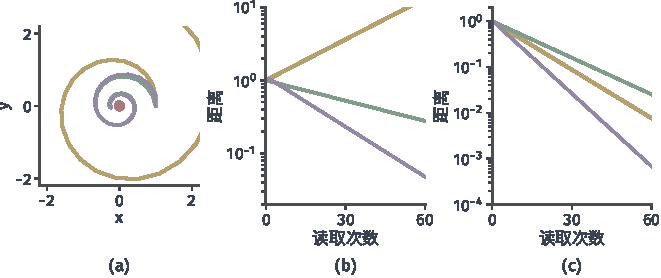
\includegraphics[width=112mm]{figures/05-optimization/07-multiple-criteria-and-nested-optimization/matplotlib/minimax-eg-paths/figure.pdf}
 \caption{三种方法的比较：黄线同时更新，绿线外梯度，紫线乐观梯度，起点$(1,0)$。(a)$f=xy$，$\alpha=0.3$，$30$轮的轨迹，红点是解。(b)$f=xy$到解的距离，横轴是方向读取次数，外梯度每轮计$2$次。(c)$f=\frac12x^2+2xy-\frac12y^2$，$\alpha=0.1$，同样按读取次数。}
 \label{fig:minimax-eg-paths}
\end{BookInlineFigure}

\subsection{乐观梯度法}
\label{sec:minimax-ogda}

\paragraph{主要思想}
外梯度法每轮读两次方向，能不能省一次？试探步的目的只是估计“下一步的方向”，而上一轮刚读过的方向已经是一个不错的估计。把试探步里的方向换成上一轮的$\bm{F}(\tilde{\bm{z}}^{(t-1)})$，无约束时得到
\[
 \tilde{\bm{z}}^{(t)}=\bm{z}^{(t)}-\alpha\bm{F}(\tilde{\bm{z}}^{(t-1)}),\qquad\bm{z}^{(t+1)}=\bm{z}^{(t)}-\alpha\bm{F}(\tilde{\bm{z}}^{(t)}).
\]
每轮只新读$\bm{F}(\tilde{\bm{z}}^{(t)})$一次。

把这个递推写成只含$\tilde{\bm{z}}$的形式。下一轮的试探点是
\[
 \tilde{\bm{z}}^{(t+1)}=\bm{z}^{(t+1)}-\alpha\bm{F}(\tilde{\bm{z}}^{(t)})=\bm{z}^{(t)}-2\alpha\bm{F}(\tilde{\bm{z}}^{(t)}).
\]
又由试探步，
\[
 \bm{z}^{(t)}=\tilde{\bm{z}}^{(t)}+\alpha\bm{F}(\tilde{\bm{z}}^{(t-1)}).
\]
代入后把$\tilde{\bm{z}}$重新记作$\bm{z}$，得到\term{乐观梯度下降—上升}（optimistic gradient descent--ascent，OGDA）：
\begin{equation}
 \bm{z}^{(t+1)}=\bm{z}^{(t)}-2\alpha\bm{F}(\bm{z}^{(t)})+\alpha\bm{F}(\bm{z}^{(t-1)}).
 \label{eq:minimax-ogda}
\end{equation}

把它写成
\[
 \bm{z}^{(t+1)}=\bm{z}^{(t)}-\alpha\bm{F}(\bm{z}^{(t)})-\alpha\bigl(\bm{F}(\bm{z}^{(t)})-\bm{F}(\bm{z}^{(t-1)})\bigr)
\]
就能看出它的含义。括号里是方向场在上一步中的变化量，代表耦合带来的转动。它按当前的变化趋势，把下一步的方向提前校正。“乐观”指相信方向场短期内的变化趋势会延续。它与重球动量的区别在于，重球叠加的是位置的差，这里叠加的是方向的差。

\paragraph{计算过程}
用$f=xy$，$\bm{F}(x,y)=(y,-x)$。

\needspace{6\baselineskip}
\paragraph{变量}
\begin{itemize}
 \item $\bm{z}^{(t)}$：当前点；
 \item $\bm{F}^{(t-1)}$：上一轮读到的方向，需要存储；
 \item $\alpha>0$：步长。
\end{itemize}

\paragraph{初始化}
取$\bm{z}^{(0)}$，并令$\bm{z}^{(-1)}=\bm{z}^{(0)}$，于是第一步就是普通的梯度步。例中$\bm{z}^{(0)}=(1,0)$，$\alpha=0.2$。

\needspace{6\baselineskip}
\paragraph{每轮更新}
\begin{enumerate}
 \item 读取当前方向$\bm{F}^{(t)}=\bm{F}(\bm{z}^{(t)})$。例中第一轮$\bm{F}^{(0)}=(0,-1)$，第二轮
 \[
  \bm{z}^{(1)}=(1,0.2),\qquad\bm{F}^{(1)}=(0.2,-1).
 \]
 \item 由式~\eqref{eq:minimax-ogda}更新，并保存$\bm{F}^{(t)}$。例中第二轮
 \[
  \bm{z}^{(2)}=(1,0.2)-0.4(0.2,-1)+0.2(0,-1)=(0.92,0.4).
 \]
\end{enumerate}

继续计算，得到
\[
 \bm{z}^{(3)}=(0.8,0.568),\qquad\bm{z}^{(4)}=(0.6528,0.704).
\]
距离的平方依次为$1,1.04,1.0064,0.9626,0.9218$，第一步因为没有历史而外漂，之后开始收缩。最终得到的迭代点沿螺旋线趋向鞍点，每轮只读一次方向。

\paragraph{双线性情形的稳定性}
线性的$\bm{F}$可以算到底。把$(x,y)$看作复数$w=x+\mathrm{i}y$，$\bm{F}=(y,-x)$对应$-\mathrm{i}w$，同时更新就成了$w^{+}=(1+\mathrm{i}\alpha)w$，与式~\eqref{eq:minimax-gda-growth}一致。式~\eqref{eq:minimax-ogda}成为二阶递推
\[
 w^{(t+1)}=(1+2\mathrm{i}\alpha)w^{(t)}-\mathrm{i}\alpha w^{(t-1)}.
\]
它的特征方程是$s^2-(1+2\mathrm{i}\alpha)s+\mathrm{i}\alpha=0$，判别式是
\[
 (1+2\mathrm{i}\alpha)^2-4\mathrm{i}\alpha=1-4\alpha^2.
\]

$0<\alpha\leq\frac12$时判别式非负，两根是$\frac12(1+2\mathrm{i}\alpha\pm\sqrt{1-4\alpha^2})$，模较大的那个满足
\begin{equation}
 \rho^2=\frac{1+\sqrt{1-4\alpha^2}}{2}<1.
 \label{eq:minimax-ogda-bilinear}
\end{equation}

$\alpha=0.2$时$\rho^2\approx0.958$，上面逐步算出的距离确实以这个比例下降。小步长时$\rho^2\approx1-\alpha^2$，和外梯度的式~\eqref{eq:minimax-eg-contraction}同阶。$\alpha>\frac12$时两根的虚部不同，由$\lvert s\rvert^2<1$可得稳定的条件是$\alpha<1/\sqrt{3}\approx0.577$，见图~\ref{fig:minimax-ogda-stability}(a)。外梯度的范围更宽，到$\alpha<1$。

\begin{BookInlineFigure}
 \centering
 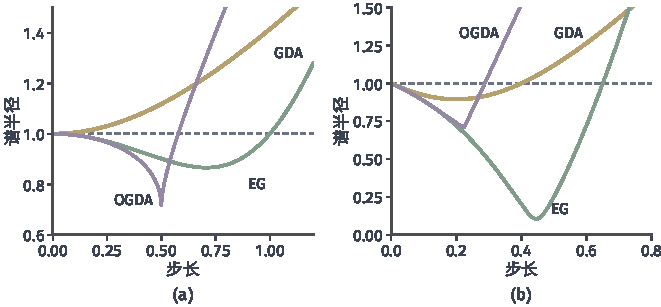
\includegraphics[width=112mm]{figures/05-optimization/07-multiple-criteria-and-nested-optimization/matplotlib/minimax-ogda-stability/figure.pdf}
 \caption{线性$\bm{F}$上的谱半径与步长的关系。虚线是稳定边界$1$。(a)$f=xy$：同时更新（GDA）全在边界之上。外梯度（EG）到$\alpha<1$稳定，乐观梯度（OGDA）到$\alpha<0.577$稳定。(b)$f=\frac12x^2+2xy-\frac12y^2$：三种方法都有稳定区间，分别到$0.4$、$0.65$、$0.29$。}
 \label{fig:minimax-ogda-stability}
\end{BookInlineFigure}

\paragraph{强凸—强凹情形}
取$f=\frac12x^2+2xy-\frac12y^2$，关于$x$强凸，关于$y$强凹，$\mu=1$。$\bm{F}$是线性的，其矩阵的特征值和Lipschitz常数是
\[
 \lambda=1\pm2\mathrm{i},\qquad L=\lvert\lambda\rvert=\sqrt5.
\]

同时更新和外梯度的每轮因子分别是$\lvert1-\alpha\lambda\rvert$和$\lvert1-\alpha\lambda+\alpha^2\lambda^2\rvert$。乐观梯度的因子是下面方程模较大的根：\[
 s^2-(1-2\alpha\lambda)s-\alpha\lambda=0.
\]

\begin{BookInlineTable}
 \centering
 \begin{tabular}{@{}llll@{}}
  \toprule
  方法 & $\alpha=0.1$ & $\alpha=0.2$ & 稳定上限\\
  \midrule
  GDA & $0.922$ & $0.894$ & $0.400$\\
  EG & $0.885$ & $0.721$ & $0.651$\\
  OGDA & $0.885$ & $0.739$ & $0.288$\\
  \bottomrule
 \end{tabular}
 \caption{$f=\frac12x^2+2xy-\frac12y^2$上三种方法的每轮收缩因子及步长上限（数值求得）。}
 \label{tab:minimax-sc-rates}
\end{BookInlineTable}

表~\ref{tab:minimax-sc-rates}的因子是按轮计算的，外梯度每轮读两次方向。按读取次数折算，$\alpha=0.1$时外梯度相当于每次读取收缩$\sqrt{0.885}\approx0.941$，比同时更新的$0.922$还慢，图~\ref{fig:minimax-eg-paths}(c)里绿线在黄线之上就是这个原因。外梯度的优势要靠较大的步长才能体现，图~\ref{fig:minimax-ogda-stability}(b)中它在$\alpha\approx0.45$处的每轮因子只有$0.105$。

对一般的强单调、Lipschitz算子，已知结论是外梯度和乐观梯度取$\alpha$为$1/L$量级时，每轮收缩因子是$1-O(\mu/L)$，而同时更新的步长要小到$\mu/L^2$量级，因子是$1-O(\mu^2/L^2)$。证明需要构造带历史项的势函数，篇幅较长，读者可查阅专门的变分不等式著作。

\paragraph{不能直接推广的情形}
上述核对都在单调问题上。$f=y^2-x^2$的$\bm{F}=(-2x,-2y)$，$\lambda=-2$，原点是排斥的：式~\eqref{eq:minimax-ogda}的特征方程$s^2-(1+4\alpha)s+2\alpha=0$在$s=1$处取值$-2\alpha<0$，所以有一根大于$1$。同样的计算也使外梯度的因子$1+2\alpha+4\alpha^2$大于$1$。

有约束时还要分清变体。把投影直接加到式~\eqref{eq:minimax-ogda}上，得到$P_{\bm{Z}}(\bm{z}^{(t)}-2\alpha\bm{F}(\bm{z}^{(t)})+\alpha\bm{F}(\bm{z}^{(t-1)}))$；另一种形式保留试探点和校正点两条序列，各做一次投影。无约束时二者等价，有约束时不是同一个递推。

例如在盒子$[-1,1]^2$上，$\bm{z}^{(0)}=(1,0.9)$，$\alpha=0.4$，$\bm{F}=(y,-x)$，第一步前者给出$(0.64,1)$，后者给出$(0.6,1)$。两种形式的步长条件和分析要分别核对，不能把其中一种的保证直接用到另一种，更不能推广到任意的非凸问题。

\section{结果评价}
\label{sec:minimax-evaluation}

算法停下来，交出一对$(\bm{x},\bm{y})$，它有多好？极小极大问题里，$f(\bm{x}^{(t)},\bm{y}^{(t)})$的升降不能回答这个问题，图~\ref{fig:minimax-gda-monitor}已经表明，两侧的优化方向本来相反，这个数上下波动没有确定的含义。

所以第一步是说清要评价什么。表~\ref{tab:minimax-evidence}按目标列出相应的证据。

\begin{BookInlineTable}
 \centering
 \begin{tabular}{@{}lll@{}}
  \toprule
  目标 & 证据 & 成立前提\\
  \midrule
  全局鞍点 & 间隙$G$或其有效上界 & 两侧极值能算或能界\\
  值函数最小 & $\phi$的（次）梯度 & 内层响应可信\\
  局部结构 & 二阶条件 & 只在邻域内有意义\\
  \bottomrule
 \end{tabular}
 \caption{评价目标与相应的证据。}
 \label{tab:minimax-evidence}
\end{BookInlineTable}

\subsection{误差证据}
\label{sec:minimax-error-evidence}

凸凹问题上最好的证据是间隙~\eqref{eq:minimax-gap}。若$\phi$和$\psi$能直接算出，例如$f$双线性而$\bm{X},\bm{Y}$是单纯形或盒子，内层就是线性函数在顶点上取值，这时间隙是精确的。

\paragraph{平均点与最后一点}
定理~\ref{thm:minimax-eg-gap}保证的是平均点。最后一点可能完全不同。在盒子$[-1,1]^2$上，$f=xy$，$L=1$，取外梯度法的边界步长$\alpha=1$，从$(1,0)$出发。第一轮试探点和校正点是
\[
 \tilde{\bm{z}}^{(0)}=(1,1),\qquad\bm{z}^{(1)}=(1,0)-(1,-1)=(0,1).
\]
继续下去，$\bm{z}^{(t)}$依次经过$(1,0),(0,1),(-1,0),(0,-1)$，每四轮回到起点。试探点依次是四个顶点。

由式~\eqref{eq:minimax-box-gap}，最后一点的间隙恒为$1$，没有收敛。而试探点的平均，$T=1,2,3,4$时间隙分别是$2,1,\frac23,0$，都不超过定理的上界$\frac{D^2}{2\alpha T}=\frac4T$，这里$D^2=8$，见图~\ref{fig:minimax-average-last}。

\begin{BookInlineFigure}
 \centering
 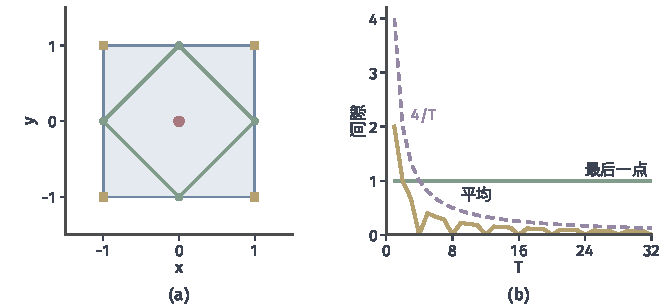
\includegraphics[width=112mm]{figures/05-optimization/07-multiple-criteria-and-nested-optimization/matplotlib/minimax-average-last/figure.pdf}
 \caption{外梯度法取边界步长$\alpha=1/L=1$，$f=xy$，$\bm{Z}=[-1,1]^2$，起点$(1,0)$。(a)绿点是校正点，沿菱形循环；黄色方块是试探点，在四个顶点循环；红点是鞍点。(b)绿线是最后一点的间隙，恒为$1$；黄线是试探点平均的间隙，在每四轮的整数倍处为$0$；紫色虚线是上界$4/T$。}
 \label{fig:minimax-average-last}
\end{BookInlineFigure}

$\alpha<1/L$时可以证明校正点本身收敛到某个鞍点，这个例子的循环出现在边界步长上。最后一点的间隙速率比平均点慢，一般是$O(1/\sqrt{T})$，证明较长，读者可查阅外梯度法最后迭代分析的专门文献。报告结果时要说清楚输出的是平均点还是最后一点，因为定理的结论只属于它所针对的那一个。

\paragraph{近似内层给出的间隙偏小}
$\phi$和$\psi$算不出来时，通常用内层算法分别求一个近似响应$\tilde{\bm{y}}$和近似外层点$\tilde{\bm{x}}$，然后计算
\begin{equation}
 \hat{G}=f(\bm{x},\tilde{\bm{y}})-f(\tilde{\bm{x}},\bm{y}).
 \label{eq:minimax-gap-estimate}
\end{equation}

因为$f(\bm{x},\tilde{\bm{y}})\leq\phi(\bm{x})$，$f(\tilde{\bm{x}},\bm{y})\geq\psi(\bm{y})$，所以$\hat{G}\leq G$。这与第~\ref{chap:duality}章“内层近似的方向”是同一个现象，误差方向正好不利：内层算得越粗糙，估计的间隙越小，算法看起来越好。

取盒子上的$f=xy$，候选$(x,y)=(0.4,-0.2)$，由式~\eqref{eq:minimax-box-gap}，真实间隙是$0.6$。内层只走一步步长$\frac12$的投影梯度：
\[
 \tilde{y}=-0.2+\frac12\cdot0.4=0,\qquad\tilde{x}=0.4-\frac12\cdot(-0.2)=0.5.
\]
式~\eqref{eq:minimax-gap-estimate}给出
\[
 \hat{G}=f(0.4,0)-f(0.5,-0.2)=0+0.1=0.1.
\]
真实间隙$0.6$被低估了六倍。

要得到可靠的上界，必须把内层误差补回去。第~\ref{chap:duality}章由梯度残差得到认证界：$\mu$强凸函数在$\tilde{\bm{x}}$处的最小值至少是函数值减去$\lVert\nabla\rVert_2^2/(2\mu)$。把它用到$-f(\bm{x},\cdot)$和$f(\cdot,\bm{y})$上。设$\bm{X}=\mathbb{R}^n$，$\bm{Y}=\mathbb{R}^q$，$f(\bm{x},\cdot)$是$\mu_y$强凹的，$f(\cdot,\bm{y})$是$\mu_x$强凸的，则
\begin{equation}
 G(\bm{x},\bm{y})\leq\hat{G}+\frac{\lVert\nabla_{\bm{y}}f(\bm{x},\tilde{\bm{y}})\rVert_2^2}{2\mu_y}+\frac{\lVert\nabla_{\bm{x}}f(\tilde{\bm{x}},\bm{y})\rVert_2^2}{2\mu_x}.
 \label{eq:minimax-certified-gap}
\end{equation}

验算一例。$f=\frac12x^2+2xy-\frac12y^2$，$\mu_x=\mu_y=1$，候选$(0.2,0.1)$。真实值由$\phi(x)=\frac52x^2$，$\psi(y)=-\frac52y^2$算出，
\[
 G=0.1+0.025=0.125.
\]

取近似响应$\tilde{y}=0.3$，$\tilde{x}=-0.1$，则
\[
 f(0.2,0.3)=0.095,\qquad f(-0.1,0.1)=-0.02,\qquad\hat{G}=0.115.
\]
两个残差是$\partial_yf(0.2,0.3)=0.1$，$\partial_xf(-0.1,0.1)=0.1$，式~\eqref{eq:minimax-certified-gap}的修正量各是$0.005$，得到上界
\[
 0.115+0.005+0.005=0.125.
\]
未修正的$\hat{G}$比真实间隙小，修正之后的上界不小于真实间隙。这里等号成立，因为函数恰好是二次的，曲率常数处处精确。

\subsection{非凸问题}
\label{sec:minimax-nonconvex}

没有凸凹性时，间隙可能恒为正，甚至恒为无穷，图~\ref{fig:minimax-saddle-types}(c)的原点就是这样。此时的目标是顺序问题本身，证据要分三层报告，各说明它证明了什么。

\paragraph{值函数的驻定证据}
内层强凹时，$\phi$可微，外层的驻定量可以由已知量给出上界。由三角不等式和式~\eqref{eq:minimax-gradient-error}，
\begin{equation}
 \lVert\nabla\phi(\bm{x})\rVert_2\leq\lVert\nabla_{\bm{x}}f(\bm{x},\tilde{\bm{y}})\rVert_2+L\sqrt{\frac{2\varepsilon}{\mu}}.
 \label{eq:minimax-stationarity-bound}
\end{equation}

用$f=-\frac12x^2+2xy-\frac12y^2$，取$x=0.1$，$\tilde{y}=0.18$。此时外层偏导数是$-0.1+0.36=0.26$，内层间隙是$\frac12(0.02)^2=0.0002$。交叉系数是$2$，第二项是$2\cdot0.02=0.04$，上界是$0.30$，真实导数$3x$也是$0.30$。

式~\eqref{eq:minimax-stationarity-bound}需要$\varepsilon$的可靠上界。内层强凹且无约束时，式~\eqref{eq:minimax-certified-gap}用到的残差界同样适用，$\varepsilon$不超过残差平方除以$2\mu$；有约束时要用相应的对偶界。

\paragraph{响应求解的证据}
内层不凹时，$\varepsilon$一般没有可计算的上界。从多个起点运行内层算法，取最大的值作为$\phi(\bm{x})$的估计，这是一个越算越大的下界。报告时要写成“在所检查的响应中最坏值是多少”，并说明检查的范围。它不是全局最坏值。式~\eqref{eq:minimax-nonconcave}在$x=1$处，从$y<-0.618$出发只能得到$0.25$，从$y>-0.618$出发才能得到$3.023$。

\paragraph{局部极小极大条件}
不要求全局最坏时，可以问一个更弱的问题：相对于局部的响应分支，当前点是不是极小？下面的二阶充分条件给出一种准确的说法。

\begin{theorem}[局部极小极大的二阶充分条件]
\label{thm:minimax-local}
设$f$在$(\bar{\bm{x}},\bar{\bm{y}})$附近二阶连续可微，$\nabla_{\bm{x}}f$和$\nabla_{\bm{y}}f$在该点为零，$\nabla^2_{\bm{y}\bm{y}}f\prec\bm{0}$，并且
\begin{equation}
 \bm{S}=\nabla^2_{\bm{x}\bm{x}}f-\nabla^2_{\bm{x}\bm{y}}f\,(\nabla^2_{\bm{y}\bm{y}}f)^{-1}\,\nabla^2_{\bm{y}\bm{x}}f\succ\bm{0}.
 \label{eq:minimax-schur}
\end{equation}
则存在定义在$\bar{\bm{x}}$某邻域上的连续可微映射$\bm{y}(\bm{x})$，$\bm{y}(\bar{\bm{x}})=\bar{\bm{y}}$，使$\bm{y}(\bm{x})$是$f(\bm{x},\cdot)$的局部极大点，且$\bar{\bm{x}}$是$\bm{x}\mapsto f(\bm{x},\bm{y}(\bm{x}))$的严格局部极小点。称这样的$(\bar{\bm{x}},\bar{\bm{y}})$为\term{局部极小极大点}（local minimax point）。
\end{theorem}

\begin{proof}
方程$\nabla_{\bm{y}}f(\bm{x},\bm{y})=\bm{0}$在该点关于$\bm{y}$的Jacobian是$\nabla^2_{\bm{y}\bm{y}}f$，可逆。隐函数定理给出连续可微的$\bm{y}(\bm{x})$，其导数是
\[
 \nabla\bm{y}(\bm{x})=-(\nabla^2_{\bm{y}\bm{y}}f)^{-1}\nabla^2_{\bm{y}\bm{x}}f.
\]
由连续性，$\nabla^2_{\bm{y}\bm{y}}f$在邻域内保持负定，所以$\bm{y}(\bm{x})$是局部极大点。

令$h(\bm{x})=f(\bm{x},\bm{y}(\bm{x}))$。因为在响应分支上$\nabla_{\bm{y}}f=\bm{0}$，链式法则只留下关于$\bm{x}$的偏梯度：
\[
 \nabla h(\bm{x})=\nabla_{\bm{x}}f(\bm{x},\bm{y}(\bm{x})).
\]
再求一次导，得到
\[
 \nabla^2h=\nabla^2_{\bm{x}\bm{x}}f+\nabla^2_{\bm{x}\bm{y}}f\,\nabla\bm{y}(\bm{x}).
\]
代入$\nabla\bm{y}$的表达式，在$\bar{\bm{x}}$处就是$\bm{S}$。又$\nabla h(\bar{\bm{x}})=\bm{0}$，$\bm{S}\succ\bm{0}$，由二阶充分条件，$\bar{\bm{x}}$是$h$的严格局部极小点。
\end{proof}

对$f=-\frac12x^2+2xy-\frac12y^2$，$\nabla^2_{yy}f=-1$，$S=-1-2\cdot(-1)\cdot2=3$，恰好是$\phi''$。

这个条件只回答局部响应分支。把式~\eqref{eq:minimax-nonconcave}放到$(1,-1)$处，两个偏导数$x+y$和$x+2y-y^3$都是$0$，$\partial_y^2f=2-3y^2=-1<0$，$\partial_x^2f=1$，$\partial_{xy}f=1$，
\[
 S=1-1\cdot(-1)\cdot1=2>0.
\]
定理的全部条件都满足，$(1,-1)$是局部极小极大点。可是$\phi'(1)=2.618\neq0$，$\phi(1)=3.023$，而外层真正的最优解是$x=0$。局部极小极大是相对于“内层只能看到附近”这个模型的结论，不能当作原问题的解来报告。

\paragraph{计算预算}
不同方法每轮的工作量相差悬殊，一轮精确内解和一轮下降—上升不能直接比较。图~\ref{fig:minimax-budget}是同一组运行的两种画法。(a)按外层轮数，$K=1$明显落后，$K=10$几乎与精确响应重合，$K=3$在这组系数下收缩最快；(b)按梯度读取总数，$K=10$反而最慢，因为它每轮要读$11$次。

\begin{BookInlineFigure}
 \centering
 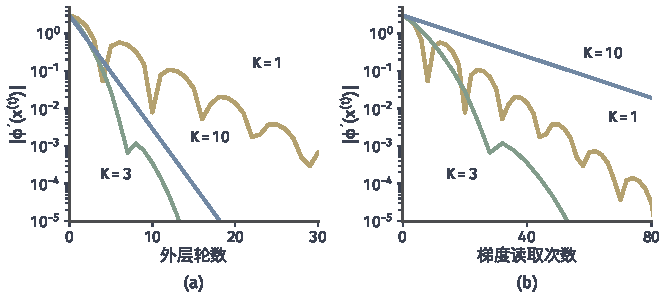
\includegraphics[width=112mm]{figures/05-optimization/07-multiple-criteria-and-nested-optimization/matplotlib/minimax-budget/figure.pdf}
 \caption{$f=-\frac12x^2+2xy-\frac12y^2$上每轮做$K$步内层上升的方法，$\alpha=\frac16$，$\beta=\frac12$，起点$(1,0)$。黄线$K=1$，绿线$K=3$，蓝线$K=10$。(a)按外层轮数，灰色虚线是精确响应。(b)同样的运行按梯度读取次数，每轮读取$K+1$次。}
 \label{fig:minimax-budget}
\end{BookInlineFigure}

报告的预算应当分开写明外层迭代次数、每次内层的计算量以及方向读取的总次数。这个例子里内层便宜且条件好，$K=3$在读取次数上最省。换一个问题，这个顺序可以完全不同。

\section{本章小结}
\label{sec:minimax-summary}

本章研究固定代价$f$下的问题$\inf_{\bm{x}}\sup_{\bm{y}}f$，它有两层结构：外层最小化，内层取最坏情形。开头的三个困难，分别由最坏值函数、鞍点和更新动力学来回答，这三者回答的是不同的问题。

\begin{BookInlineTable}
 \centering
 \begin{tabular}{@{}lll@{}}
  \toprule
  工具 & 回答的问题 & 依赖的条件\\
  \midrule
  最坏值函数$\phi$ & 外层在最小化什么 & $\bm{Y}$紧时连续，响应唯一时可微\\
  全局鞍点与间隙 & 一对候选是否全局解 & 紧凸且凸凹时存在\\
  迭代动力学 & 算法会不会靠近解 & 单调性、Lipschitz性、步长\\
  \bottomrule
 \end{tabular}
 \caption{本章的三个主要工具。}
 \label{tab:minimax-summary}
\end{BookInlineTable}

顺序极小极大问题与同时下降—上升算法是两回事。前者是要解的数学问题，后者是一种迭代格式。图~\ref{fig:minimax-saddle-types}(c)的原点是顺序问题的解，却不是鞍点；$f=xy$上的同时更新发散，问题本身却有鞍点。

判断一个结果可信，要分别核对四项条件：
\begin{enumerate}
 \item 最值交换。只有凸凹性和相应的紧性成立时才能交换$\inf$和$\sup$，值相等还要另外核对达到，才有鞍点。
 \item 内层准确性。Danskin公式要全局最优响应，局部极大不能代替。强凹时内层间隙能转成外层梯度的误差，非凹时梯度残差小不保证接近最坏值。
 \item 耦合迭代的稳定。反对称的耦合产生旋转，下降—上升在双线性问题上不收敛。内层强凹时要让$\bm{y}$跟得上，单调问题上可以用外梯度或乐观梯度校正方向。
 \item 最终误差。间隙是全局证书，但只用近似内层算出的间隙偏小，需要修正；限定间隙和局部二阶条件都不能冒充全局结论。
\end{enumerate}

本章两层共用同一个代价$f$，内层想让$f$大，外层想让$f$小。下一章的两层目标各不相同，外层依赖内层的最优解，那时值函数的导数不再由这样简单的公式给出。

